% !TeX document-id = {d83918a8-c659-4a46-8234-071d697471ea}
% !TeX TXS-program:compile = txs:///xelatex/[--shell-escape]
% !TeX TXS-program:bibliography = txs:///biber

%%%%%%%%%%%%%%%%%%%%%%%%%%%%%%%%%%%%%%%%%%%%%%%%%%%%%%%%%%%%%%%%%%%%%%%%%%%%%%%%
%% Plantilla de memoria en LaTeX para TFG/TFM - Universidad Rey Juan Carlos
%%
%% Por Gregorio Robles <grex arroba gsyc.urjc.es>
%%     Felipe Ortega   <felipe.ortega@urjc.es>
%%     Grupo de Sistemas y Comunicaciones (GSyC)
%%     Escuela Técnica Superior de Ingenieros de Telecomunicación
%%     Universidad Rey Juan Carlos
%%
%% (Muchas ideas tomadas de Internet, colegas del GSyC, antiguos alumnos...
%%  etc. Muchas gracias a todos)
%%
%% La última versión de esta plantilla está siempre disponible en:
%%     https://github.com/glimmerphoenix/plantilla-memoria
%%
%% - Ejecución en sistema local:
%% Para obtener el documento en PDF, ejecuta en la shell:
%%   make
%%
%% A diferencia de la anterior versión, que usaba la herramienta pdfLaTeX 
%% para compilar el documento, esta nueva versión de la plantilla usa
%% XeLaTeX. Es un compilador más moderno que, entre otras mejoras, incluye
%% soporte nativo para caracteres con codificación UTF-8, traducción políglota
%% de referencias (usando Biblatex) y soporte para fuentes OTF. Esta última
%% característic permite, por ejemplo, insertar iconos de la colección 
%% Fontawesome en el texto.
%%
%% XeLaTeX viene ya incluido en todas las distribuciones modernas de LaTeX.
%%
%% - Edición y ejecución en línea: 
%% Puedes descargar y subir la plantilla a
%% Overleaf, un editor de LaTeX colaborativo en línea. Overleaf ya tiene
%% instalados todos los paquetes LaTeX y otras dependencias software para
%% que esta plantilla compile correctamente.
%%
%% IMPORTANTE: Si compilas este documento en Overleaf, recuerda cambiar
%% la configuración (botón "Menu" en la esquina superior izquierda de la interfaz)
%% y elegir la opción Compiler --> XeLaTeX. En caso contrario no funcionará.
%%
%% - Nota: las imágenes deben ir en PNG, JPG, EPS o PDF. También se pueden usar
%% imágenes en otros formatos con algunos cambios en el preámbulo del documento.

%%%%%%%%%%%%%%%%%%%%%%%%%%%%%%%%%%%%%%%%%%%%%%%%%%%%%%%%%%%%%%%%%%%%%%%%%%%%%%%%

\documentclass[a4paper, 12pt]{book}

%%-- Geometría principal (dejar activada la siguiente línea en la versión final)
\usepackage[a4paper, left=2.5cm, right=2.5cm, top=3cm, bottom=3cm]{geometry}
%%-- Activar esta línea y comentar la anterior en modo borrador, para comentarios al margen
%\usepackage[a4paper, left=2.5cm, right=2.5cm, top=3cm, bottom=3cm, marginparwidth=60pt]{geometry}

%%-- Hay que cargarlo antes que las traducciones
\usepackage{listing}                    % Listados de código

% Traducciones en XeLaTeX
\usepackage{polyglossia}
\setmainlanguage{spanish}    % Comenta esta línea si tu memoria es en inglés

% Traducciones particulares para español
% Caption tablas
\gappto\captionsspanish{
	\def\tablename{Tabla}
	\def\listingscaption{Código}
	\def\refname{Bibliografía}
	\def\appendixname{Apéndice}
	\def\listtablename{Índice de tablas}
	\def\listingname{Código}
	\def\listlistingname{Índice de fragmentos de código}
}

%% Tipografía y estilos
\usepackage[OT1]{fontenc}               % Keeps eulervm happy about accents encoding

% Símbolos y fuentes matemáticas elegantes: Euler virtual math fonts
% ¡Importante! Carga siempre las fuentes math AMS Euler ANTES QUE fontspec
\usepackage{amsmath}
\usepackage{amssymb}
\usepackage[OT1,euler-digits,euler-hat-accent,small]{eulervm}

% En XeLaTeX las fuentes se especifican con fontspec
\usepackage{fontspec}
\defaultfontfeatures{Scale=MatchLowercase, Ligatures=TeX}     % Default option in font config

% Fix para fuentes usadas con operadores y \mathrm
\DeclareSymbolFont{operators}{\encodingdefault}{\familydefault}{m}{n}

% Configura la fuente principal (serif): MinionPro
\setmainfont[Scale=0.96]{TeX Gyre Pagella}
% Configura la fuente sans-serif (\sffamily)
\setsansfont[Scale=MatchLowercase]{Lato}
% Configura la fuente para letra monoespaciada: Source Code Pro, escala 0.85
\setmonofont[Scale=0.85]{Source Code Pro}

%%-- Familias de fuentes específic¢as
%%-- Se pueden definir etiquetas para familias de fuentes personalizadas
%%-- que luego puedes emplear para cambiar el formato de una parte de texto
%%-- Ejemplo:
% \newfontfamily{\myriadprocond}{Myriad Pro Semibold Condensed.otf}

%%-- Opciones de interlineado y espacios
\linespread{1.07}                   % Aumentar interlineado para fuentes tipo Palatino
\setlength{\parskip}{\baselineskip} % Separar párrafos con línea en blanco

%%-- Hipervínculos
\usepackage{url}

%%-- Gráficos y tablas
\PassOptionsToPackage{
    dvipdfmx,usenames,dvipsnames,
    x11names,table}{xcolor}             % Definiciones de colores
\PassOptionsToPackage{xetex}{graphicx}

\usepackage{subfig}                     % Subfiguras
\usepackage{pgf}
\usepackage{svg}                        % Integración de imágenes en formato SVG
\usepackage{float}                      % H para posicionar figuras
\usepackage{booktabs}                   % Already loads package xcolor
\usepackage{multicol}                   % multiple column layout facilities
\usepackage{colortbl}                   % For coloured tables

%%-- Bibliografía con Biblatex y Biber
% Más info:
% https://www.overleaf.com/learn/latex/Biblatex_bibliography_styles
% https://www.overleaf.com/learn/latex/biblatex_citation_styles
\usepackage[
    backend=biber,
    style=numeric,
    sorting=nty
    ]{biblatex}
\addbibresource{memoria.bib}
\DeclareFieldFormat{url}{\mkbibacro{URL}\addcolon\nobreakspace\url{#1}}
%\usepackage[nottoc, notlot, notlof, notindex]{tocbibind} %% Opciones de índice

%%-- Matemáticas e ingeniería
% El paquete units permite mostrar unidades correctamente
% Permite escribir unidades con espaciado y estilo de fuente correctos
\usepackage[ugly]{units}         
% Ejemplo de uso: $\unit[100]{m}$ or $\unitfrac[100]{m}{s}$
% Entornos matemáticos
\newtheorem{theorem}{Theorem}

% Paquetes adicionales
\usepackage{url}                        %% Gestión correcta de enlaces
\usepackage{float}                      %% H para posicionar figuras
\usepackage[nottoc, notlot, notlof, notindex]{tocbibind}    %% Opciones de índice
\usepackage{metalogo}                   %% Múltiples logos para XeLaTeX

% Fuentes especiales y glifos
\usepackage{ccicons}                % Creative Commons icons
\usepackage{metalogo}               % XeTeX logo
\usepackage{fontawesome5}           % Fontawesome 5 icons
\usepackage{adforn} 

% Blindtext
% Opciones pangram, bible, random (defecto)
\usepackage[pangram]{blindtext}
% Lorem ipsum
\usepackage{lipsum}
% Kant lipsum
\usepackage{kantlipsum}

\usepackage{fancyvrb}               % Entornos verbatim extendidos
	\fvset{fontsize=\normalsize}    % Tamaño de fuente por defecto en fancy-verbatim
	
% Configura listas (itemize, enumerate) con iconos personalizados
% Fácil reinicio de numeración con enumerate
% Info: http://ctan.org/pkg/enumitem
\usepackage[shortlabels]{enumitem}
% Usar \usageitem para configurar iconos personalizados en listas
\newcommand{\usageitem}[1]{%
	\item[%
	{\makebox[2em]{\strut\color{GSyCblue} #1}}%
	]
}

%%-- Definición de colores personalizados
% \definecolor{LightGrey}{HTML}{EEEEEE}
% \definecolor{darkred}{rgb}{0.5,0,0}     %% Refs. cruzadas
% \definecolor{darkgreen}{rgb}{0,0.5,0}   %% Citas bibliográficas
% \definecolor{darkblue}{rgb}{0,0,0.5}    %% Hiperenlaces ordinarios (también ToC)

%%-- Configuración fragmentos de código
%%-- Minted necesita Python Pygments instalado en el sistema para funcionar
%%-- En Overleaf ya está instalada esta dependencia
% \usepackage[center, labelfont=bf]{caption}
\usepackage{minted}

%%-- Se debe cargar aquí para evitar warnings
\usepackage{csquotes}                   % Para traducciones con biblatex

%%-- Glosario de términos
\usepackage[acronym]{glossaries}
\makeglossaries
\loadglsentries{glossary}

% % Definición de cabeceras del documento, usando fancyhdr
% \usepackage{fancyhdr}
% %% Configuración de cabeceras para el cuerpo principal del documento
% \pagestyle{fancy}
% \fancyhead{}
% \fancyhead[RO,LE]{\myriadprocond{\thepage}}
% \renewcommand{\chaptermark}[1]{\markboth{\chaptername\ \thechapter.\ #1}{}}
% \renewcommand{\sectionmark}[1]{\markright{\thesection.\ #1}}
% \fancyhead[RE]{\myriadprocond{\leftmark}}
% \fancyhead[LO]{\myriadprocond{\rightmark}}
% \renewcommand{\headrulewidth}{0pt}
% \setlength{\headheight}{15pt} %% Al menos 15pt para evitar warning al compilar
% \fancyfoot{}
% %% Configuración para páginas con cabecera en blanco
% \fancypagestyle{plain}{%
% \fancyhf{}% clear all header and footer fields
% \fancyhead[RO,LE]{\myriadprocond{\thepage}}
% \renewcommand{\headrulewidth}{0pt}%
% \renewcommand{\footrulewidth}{0pt}%
% }

%%-- Metadatos del doc
\title{Memoria del Proyecto}
\author{Nombre del autor}

%%-- Hiperenlaces, siempre se carga al final del preámbulo
\usepackage[colorlinks]{hyperref}
\hypersetup{
    pdftoolbar=true,	% Muestra barra de herramientas en Adobe Acrobat
	pdfmenubar=true,	% Muestra menú en Adobe Acrobat
	pdftitle={Título doc en ventana del visor o navegador},
	pdfauthor={Nombre del alumno/a},
	pdfcreator={ETSII/ETSIT, URJC},
	pdfproducer={XeLaTeX},
	pdfsubject={Topic1, Topic2, Topic3},
	pdfnewwindow=true,              %links open in new window
    colorlinks=true,                % false: boxed links; true: coloured links
    linkcolor=Firebrick4,           % enlaces internos 
    citecolor=Aquamarine4,          % enlaces a citas bibliográficas
    urlcolor=RoyalBlue3,            % hiperenlances ordinarios
    linktocpage=true                % Enlaces en núm. pág. en ToC
}

%%%---------------------------------------------------------------------------
% Comentarios en línea de revisión
% Este bloque se puede borrar cuando finalizamos el borrador

% \usepackage[colorinlistoftodos]{todonotes}
% \usepackage{verbatim}
%%%---------------------------------------------------------------------------

\begin{document}

%%-- Configuración común para todos los entornos listing
%%-- Descomentar para usar y personalizar valores
%\lstset{%
%breakatwhitespace=true,
% breaklines=true, 
% basicstyle=\footnotesize\ttfamily,
% keywordstyle=\color{blue},
% commentstyle=\color{green!40!black}, 
% language=Python} 
 

%%%%%%%%%%%%%%%%%%%%%%%%%%%%%%%%%%%%%%%%%%%%%%%%%%%%%%%%%%%%%%%%%%%%%%%%%%%%%%%%
% PORTADA

\begin{titlepage}
\begin{center}
\begin{tabular}[c]{c c}
%
\includegraphics[bb=0 0 194 352, scale=0.25]{logo} &
\includegraphics[scale=1.5]{img/LogoURJC.png}
%&
%\begin{tabular}[b]{l}
%\Huge
%\textsf{UNIVERSIDAD} \\
%\Huge
%\textsf{REY JUAN CARLOS} \\
%\end{tabular}
\\
\end{tabular}

\vspace{3cm}

\Large 
INGENIERÍA EN TECNOLOGÍAS DE LA TELECOMUNICACIÓN

\vspace{0.4cm}

\large
Curso Académico 2024/2025

\vspace{0.8cm}

Trabajo Fin de Grado

\vspace{2cm}

\LARGE ANÁLISIS DE PATRONES DE ACTIVIDAD DE USUARIOS EN UNA PLATAFORMA WEB \\
PARA DESARROLLO DE PROYECTOS DE ROBÓTICA
\vspace{3cm}

\large
Autor/a : Alejandro Aguilera López \\
Tutor/a : José Felipe Ortega Soto
\end{center}
\end{titlepage}

\newpage
\mbox{}
\thispagestyle{empty} % para que no se numere esta pagina


%%%%%%%%%%%%%%%%%%%%%%%%%%%%%%%%%%%%%%%%%%%%%%%%%%%%%%%%%%%%%%%%%%%%%%%%%%%%%%%%
%%%% Para firmar
\clearpage
\pagenumbering{gobble}
\chapter*{}

\vspace{-4cm}
\begin{center}
\LARGE
\textbf{Trabajo Fin de Grado}

\vspace{1cm}
\large
Título del Trabajo con Letras Capitales para Sustantivos y Adjetivos

\vspace{1cm}
\large
\textbf{Autor/a :} Alejandro Aguilera López  \\
\textbf{Tutor/a :} José Felipe Ortega Soto

\end{center}

\vspace{1cm}
La defensa del presente Proyecto Fin de Grado/Máster se realizó el día 3\qquad$\;\,$ de
\qquad\qquad\qquad\qquad \newline de 20XX, siendo calificada por el siguiente tribunal:


\vspace{0.5cm}
\textbf{Presidente:}

\vspace{0.8cm}
\textbf{Secretario:}

\vspace{0.8cm}
\textbf{Vocal:}


\vspace{0.8cm}
y habiendo obtenido la siguiente calificación:

\vspace{0.8cm}
\textbf{Calificación:}


\vspace{0.8cm}
\begin{flushright}
Móstoles/Fuenlabrada, a \qquad$\;\,$ de \qquad\qquad\qquad\qquad de 20XX
\end{flushright}

%%%%%%%%%%%%%%%%%%%%%%%%%%%%%%%%%%%%%%%%%%%%%%%%%%%%%%%%%%%%%%%%%%%%%%%%%%%%%%%%
%%%% Dedicatoria

\chapter*{}
%\pagenumbering{Roman} % para comenzar la numeración de paginas en numeros romanos
\begin{flushright}
\textit{Aquí normalmente \\
se inserta una dedicatoria corta \\}
\end{flushright}

%%%%%%%%%%%%%%%%%%%%%%%%%%%%%%%%%%%%%%%%%%%%%%%%%%%%%%%%%%%%%%%%%%%%%%%%%%%%%%%%
%%%% Agradecimientos

\chapter*{Agradecimientos}
%\addcontentsline{toc}{chapter}{Agradecimientos} % si queremos que aparezca en el índice
\markboth{AGRADECIMIENTOS}{AGRADECIMIENTOS} % encabezado 

Aquí vienen los agradecimientos\ldots

Hay más espacio para explayarse y explicar a quién agradeces su apoyo o ayuda para
haber acabado el proyecto: familia, pareja, amigos, compañeros de clase\ldots

También hay quien, en algunos casos, hasta agradecer a su tutor o tutores del proyecto
la ayuda prestada\ldots

%%%%%%%%%%%%%%%%%%%%%%%%%%%%%%%%%%%%%%%%%%%%%%%%%%%%%%%%%%%%%%%%%%%%%%%%%%%%%%%%
%%%% Resumen

\chapter*{Resumen}
%\addcontentsline{toc}{chapter}{Resumen} % si queremos que aparezca en el índice
\markboth{RESUMEN}{RESUMEN} % encabezado

Aquí viene un resumen del proyecto.
Ha de constar de tres o cuatro párrafos, donde se presente de manera clara y concisa de qué va el proyecto. 
Han de quedar respondidas las siguientes preguntas:

\begin{itemize}
  \item ¿De qué va este proyecto? ¿Cuál es su objetivo principal?
  \item ¿Cómo se ha realizado? ¿Qué tecnologías están involucradas?
  \item ¿En qué contexto se ha realizado el proyecto? ¿Es un proyecto dentro de un marco general?
\end{itemize}

Lo mejor es escribir el resumen al final.

%%%%%%%%%%%%%%%%%%%%%%%%%%%%%%%%%%%%%%%%%%%%%%%%%%%%%%%%%%%%%%%%%%%%%%%%%%%%%%%%
%%%% Resumen en inglés

\chapter*{Summary}
%\addcontentsline{toc}{chapter}{Summary} % si queremos que aparezca en el índice
\markboth{SUMMARY}{SUMMARY} % encabezado

Here comes a translation of the ``Resumen'' into English. 
Please, double check it for correct grammar and spelling.
As it is the translation of the ``Resumen'', which is supposed to be written at the end, this as well should be filled out just before submitting.

%%%%--------------------------------------------------------------------
% Lista de comentarios de revisión
% Se puede borrar este bloque al acabar el borrador

%\listoftodos
%\markboth{TODO LIST}{TODO LIST} % encabezado
%%%%--------------------------------------------------------------------

%%%%%%%%%%%%%%%%%%%%%%%%%%%%%%%%%%%%%%%%%%%%%%%%%%%%%%%%%%%%%%%%%%%%%%%%%%%%%%%%
%%%%%%%%%%%%%%%%%%%%%%%%%%%%%%%%%%%%%%%%%%%%%%%%%%%%%%%%%%%%%%%%%%%%%%%%%%%%%%%%
% ÍNDICES %
%%%%%%%%%%%%%%%%%%%%%%%%%%%%%%%%%%%%%%%%%%%%%%%%%%%%%%%%%%%%%%%%%%%%%%%%%%%%%%%%

% Las buenas noticias es que los índices se generan automáticamente.
% Lo único que tienes que hacer es elegir cuáles quieren que se generen,
% y comentar/descomentar esa instrucción de LaTeX.

%%-- Índice de contenidos
\tableofcontents 
\cleardoublepage
%%-- Índice de figuras
%\addcontentsline{toc}{chapter}{Lista de figuras} % para que aparezca en el indice de contenidos
\listoffigures % indice de figuras
%\cleardoublepage
%%-- Índice de tablas
%\addcontentsline{toc}{chapter}{Lista de tablas} % para que aparezca en el indice de contenidos
%\listoftables % indice de tablas
\cleardoublepage
%%-- Índice de fragmentos de código
\listoflistings

%%%%%%%%%%%%%%%%%%%%%%%%%%%%%%%%%%%%%%%%%%%%%%%%%%%%%%%%%%%%%%%%%%%%%%%%%%%%%%%%
%%%%%%%%%%%%%%%%%%%%%%%%%%%%%%%%%%%%%%%%%%%%%%%%%%%%%%%%%%%%%%%%%%%%%%%%%%%%%%%%
% INTRODUCCIÓN %
%%%%%%%%%%%%%%%%%%%%%%%%%%%%%%%%%%%%%%%%%%%%%%%%%%%%%%%%%%%%%%%%%%%%%%%%%%%%%%%%

\cleardoublepage
\chapter{Introducción}
\label{sec:intro}
\pagenumbering{arabic} % para empezar la numeración de página con números

Debido al avance de las tecnologías, la robótica se encuentra en constante evolución, lo que hace que cada vez la podamos ver en más sectores, desde el mundo laboral hasta en nuestro día a día. Sin embargo, el aprendizaje de la robótica es un terreno complejo, ya que para poder empezar en este campo se requiere la instalación y configuración de distintas herramientas y entornos de programación, los cuales pueden resultar bastante enrevesados, en especial a nuevos usuarios que quiere empezar en el mundo de la robótica.

Otro gran problema del aprendizaje de la robótica es el coste de un robot en el cual ir probando nuestros códigos, ya que a diferencia de otras materias la robótica es un campo que su aprendizaje es a base de prueba y error.

Este trabajo de fin de grado gira entorno a UNIBOTICS una plataforma web, que nace como solución a estos problemas. UNIBOTICS permite a los usuarios acceder a ejercicios interactivos de robótica, en los cuales podrán programar robots y poder simularlos en escenarios 3D sin la necesidad de tener el robot de forma física y sin tener que instalar ningún tipo de programa.

Sin embargo, a pesar de sus ventajas, aún existen áreas de UNIBOTICS que podrían mejorarse. Actualmente, todos los datos de  usuarios desde los códigos de programación, tiempo de actividad, tiempo de resolución de actividades y muchos otros datos más, se recogen en una base de datos del tipo PostgreSQL, pero estos datos únicamente se almacenan y no se les saca todo el potencial que podrían tener.

Dada esta situación, este proyecto quiere proporcionar una API que permita extraer y procesar estos datos. Además, se diseñarán unas Dashboards interactivas, donde se podrán ver de forma clara y detallada toda la información obtenida a través de la API.

Con la implementación de estas Dashboards se busca que los profesores puedan ver de forma rápida y sencilla el trabajo realizado por sus alumnos, lo cual les podrá facilitar la enseñanza a los alumnos de robótica.

\section{Objetivos}
\label{sec:seccion}

Esto es una sección, que es una estructura menor que un capítulo. 

Por cierto, a veces me comentáis que no os compila por las tildes.
Eso es un problema de codificación.
Al guardar el archivo, guardad la codificación de ``ISO-Latin-1'' a ``UTF-8'' (o viceversa) y funcionará.

\subsection{Objetivo general} % título de subsección (se muestra)
\label{sec:objetivo-general} % identificador de subsección (no se muestra, es para poder referenciarla)


Mi Trabajo Fin de Grado consiste en crear de una herramienta que permita extraer datos de la plataforma web UNIBOTICS y crear unos dashboards interactivos para representar esa información


\subsection{Objetivos específicos}
\label{sec:objetivos-especificos}

Los objetivos específicos se pueden entender como las tareas en las que se ha desglosado el objetivo general. Y, sí, también vienen en infinitivo.

Lo mejor suele ser utilizar una lista no numerada, como sigue:

\begin{itemize}
	\item Un objetivo específico.
	\item Otro objetivo específico.
	\item Tercer objetivo específico.
	\item \ldots
\end{itemize}

\section{Planificacion}
\label{sec:objetivos}

Rellenar alfinal

\section{Estructura del documento}
\label{sec:planificacion-temporal}

Es conveniente que incluyas una descripción de lo que te ha llevado realizar el trabajo.
Hay gente que añade un diagrama de GANTT.
Lo importante es que quede claro cuánto tiempo has consumido en realizar el TFG/TFM 
(tiempo natural, p.ej., 6 meses) y a qué nivel de esfuerzo (p.ej., principalmente los 
fines de semana).

\section{Estructura de la memoria}
\label{sec:estructura}

Por último, en esta sección se introduce a alto nivel la organización del resto del documento
y qué contenidos se van a encontrar en cada capítulo.

    \begin{itemize}
      \item En el primer capítulo se hace una breve introducción al proyecto, se describen los objetivos del mismo y se refleja la planificación temporal.
      \item En el siguiente capítulo se describen las tecnologías utilizadas en el desarrollo de este TFM/TFG (Capítulo~\ref{chap:tecnologias}).
      \item En el capítulo~\ref{chap:diseño} Se describe el proceso de desarrollo
      de la herramienta \ldots
      \item En el capítulo~\ref{chap:experimentos} Se presentan las principales pruebas realizadas
      para validación de la plataforma/herramienta\ldots (o resultados de los experimentos
      efectuados).
      \item Por último, se presentan las conclusiones del proyecto así como los trabajos futuros que podrían derivarse de éste (Capítulo~\ref{chap:conclusiones}).
    \end{itemize}

\cleardoublepage

%%%%%%%%%%%%%%%%%%%%%%%%%%%%%%%%%%%%%%%%%%%%%%%%%%%%%%%%%%%%%%%%%%%%%%%%%%%%%%%%
%%%%%%%%%%%%%%%%%%%%%%%%%%%%%%%%%%%%%%%%%%%%%%%%%%%%%%%%%%%%%%%%%%%%%%%%%%%%%%%%
% ESTADO DEL ARTE %
%%%%%%%%%%%%%%%%%%%%%%%%%%%%%%%%%%%%%%%%%%%%%%%%%%%%%%%%%%%%%%%%%%%%%%%%%%%%%%%%

\chapter{Tecnologías}               %% a.k.a "Tecnologías utilizadas"
\label{chap:tecnologias}

En este capitulo describiré las tecnologías utilizadas para este proyecto.


\section{Python}
\label{sec:python}

Python es un lenguaje de programación de alto nivel, interpretado, dinámico y fuertemente tipado. Python es un lenguaje multiparadigma, lo que quiere decir que permite desarrollar software utilizando distintos enfoques como la programación orientada a objetos, la programación funcional y la programación imperativa.

El principal motivo por el cual he elegido Python como lenguaje de programación para este trabajo es que la plataforma UNIBOTICS está desarrollada en este lenguaje, por lo que usar otro sería ineficiente y una complicación innecesaria. Además, Python destaca por su simplicidad y legibilidad, lo que facilita el desarrollo y mantenimiento del código, su gran comunidad que ofrece soporte constante y su gran variedad de bibliotecas en las cuales se apoya este proyecto. A continuación se enumeran y se detallan el funcionamiento de cada una:

\subsection{Pandas}\label{subsec:pandas}
Pandas es una de las herramientas más poderosas para la manipulación y análisis de datos en Python. Esta biblioteca se diseñó para hacer que la limpieza, transformación y análisis de datos sean rápidos y eficientes.

Una de las razones por las que he elegido pandas en este proyecto es su capacidad para manipular datos de manera flexible y eficiente. Sus estructuras principales, Series y DataFrame, facilitan la organización y el acceso a la información de manera intuitiva. La Series actúa como un array unidimensional con etiquetas asociadas, mientras que el DataFrame es una tabla bidimensional que permite realizar operaciones similares a las de bases de datos o herramientas como Excel.

En el contexto de este proyecto, pandas es la mejor opción porque la plataforma en la que se desarrollará ya está basada en Python y requiere una gestión eficiente de datos tabulares. Además, como se menciona en *Python for Data Analysis*, 3rd Edition, pandas no solo facilita la manipulación de datos, sino que también nos permite enfocarnos en la interpretación y visualización de la información, en lugar de perder tiempo en tareas repetitivas de procesamiento.

\subsection{Dash}\label{subsec:dash}
Dash es una herramienta de Python que permite crear aplicaciones web interactivas de forma sencilla. 

En este proyecto, lo he utilizado porque facilita la creación de gráficos atractivos e interactivos para visualizar los datos de la plataforma UNIBOTICS. Con Dash, puedo generar visualizaciones que permiten a los usuarios interactuar con los datos de manera intuitiva, como hacer filtros o explorar diferentes métricas. Esto es ideal para representar información compleja de forma clara y visualmente atractiva. Además, Dash se integra muy bien con otras bibliotecas de Python, lo que hace que sea fácil crear gráficos de todo tipo, desde barras hasta mapas interactivos.

\subsection{Psycopg2}\label{subsec:psycopg2}
Psycopg2 es una librería de Python que permite conectar aplicaciones Python con bases de datos PostgreSQL. Es ampliamente utilizada debido a su eficiencia y facilidad de uso para interactuar con bases de datos. 

En este proyecto, he utilizado Psycopg2 para ejecutar consultas SQL directamente desde Python, lo que permite extraer, insertar y modificar datos de manera eficiente. Esta librería ofrece una interfaz sencilla y rápida para gestionar la conexión con la base de datos y ejecutar comandos SQL de forma segura, evitando vulnerabilidades como la inyección de SQL. Además, su integración con otras bibliotecas de Python, como Pandas \ref{subsec:pandas}, facilita la manipulación y análisis de los datos obtenidos desde la base de datos, lo que hace que sea más fácil la integración con Dash \ref{subsec:dash}.


\section{PostgreSQL}
\label{sec:PostgreSQL}
PostgreSQL es un sistema de base de datos muy seguro y popular que se utiliza para guardar y organizar grandes cantidades de datos. Es de código abierto, lo que significa que cualquiera puede usarlo y adaptarlo según sus necesidades. 

Una de las razones por las que es tan utilizado es que permite hacer consultas complejas de manera rápida y segura, asegurando que los datos se mantengan intactos y bien organizados. En el caso de Unibotics, toda la información relacionada con los usuarios y sus interacciones en la plataforma se almacena en una base de datos PostgreSQL. Aunque se hablará más adelante sobre cómo está estructurada esta base de datos \ref{sec:arquitectura}, lo importante es que PostgreSQL ofrece una forma eficiente y segura de gestionar toda esa información.

\section{Docker}
\label{sec:docker}

Docker es una plataforma de virtualización ligera basada en contenedores que permite empaquetar una aplicación junto con todas sus dependencias en una única unidad portátil. Cada contenedor comparte el núcleo del sistema operativo, pero se ejecuta de forma aislada, lo que garantiza que el entorno interno sea siempre el mismo, independientemente de la máquina donde se despliegue.

En este proyecto hemos utilizado Docker principalmente para levantar la base de datos PostgreSQL de Unibotics en un contenedor independiente. De esta manera, pude iniciar, detener o reiniciar la base de datos con un solo comando, sin necesidad de instalar PostgreSQL en el sistema anfitrión ni preocuparme por posibles conflictos con otras versiones de la base de datos. Además, al usar Docker, tengo la garantía de que el entorno de ejecución es idéntico en mi máquina local y en cualquier otro entorno de pruebas o producción donde se despliegue la plataforma.


\section{Entorno de desarrollo: PyCharm}
\label{sec:entorno_de_desarrollo}

%%-- El comando \gls{} permite incluir términos en el glosario, para luego reunirlos todos
%%-- en una tabla al comienzo o al final del documento, junto con sus definiciones.

PyCharm es un \gls{ide} dedicado concretamente a la programación en Python y desarrollado por la compañía checa JetBrains.

Proporciona análisis de código, un depurador gráfico, una consola de Python integrada, control de versiones y, además, soporta desarrollo web con Django. Todas estas características lo convierten en un entorno completo e intuitivo, idóneo para el desarrollo de proyectos académicos como el que nos ocupa.


\section{Redacción de la memoria: LaTeX/Overleaf}
\label{sec:redaccion_de_la_memoria}

LaTeX es un sistema de composición tipográfica de alta calidad que incluye características especialmente diseñadas para la producción de documentación técnica y científica. Estas características, entre las que se encuentran la posibilidad de incluir expresiones matemáticas, fragmentos de código, tablas y referencias, junto con el hecho de que se distribuya como software libre, han hecho que LaTeX se convierta en el estándar de facto para la redacción y publicación de artículos académicos, tesis y todo tipo de documentos científico-técnicos. 

Por su parte, Overleaf es un editor LaTeX colaborativo basado en la nube. Lanzado originalmente en 2012, fue creado por dos matemáticos que se inspiraron en su propia experiencia en el ámbito académico para crear una solución satisfactoria para la escritura científica colaborativa.

Además de por su perfil colaborativo, Overleaf destaca porque, pese a que en LaTeX el escritor utiliza texto plano en lugar de texto formateado (como ocurre en otros procesadores de texto como Microsoft Word, LibreOffice Writer y Apple Pages), éste puede visualizar en todo momento y paralelamente el texto formateado que resulta de la escritura del código fuente.

\cleardoublepage

%%%%%%%%%%%%%%%%%%%%%%%%%%%%%%%%%%%%%%%%%%%%%%%%%%%%%%%%%%%%%%%%%%%%%%%%%%%%%%%%
%%%%%%%%%%%%%%%%%%%%%%%%%%%%%%%%%%%%%%%%%%%%%%%%%%%%%%%%%%%%%%%%%%%%%%%%%%%%%%%%
% DISEÑO E IMPLEMENTACIÓN %
%%%%%%%%%%%%%%%%%%%%%%%%%%%%%%%%%%%%%%%%%%%%%%%%%%%%%%%%%%%%%%%%%%%%%%%%%%%%%%%%

\chapter{Arquitectura}
\label{chap:diseño}


Aquí viene todo lo que has hecho tú (tecnológicamente). 
Puedes entrar hasta el detalle. 
Es la parte más importante de la memoria, porque describe lo que has hecho tú.
Eso sí, normalmente aconsejo no poner código, sino diagramas.

\section{Arquitectura general} 
\label{sec:arquitectura}

Como ya dije antes, UNIBOTICS es una plataforma web diseñada con el fin de facilitar el aprendizaje práctico de la robótica, proporcionando a los estudiantes un entorno en el que pueden encontrar ejercicios y escenarios interactivos sin la necesidad de instalar o configurar entornos complejos de software.

Esta plataforma proporciona diferentes herramientas para trabajar con robots. La herramienta que gestiona el software robótico requerido, es RADI (Robotics Academy Docker Image). Se trata de unos contenedores Docker especiales en los que se llevan a cabo la ejecución de ejercicios y las simulaciones robóticas.

Estos contenedores integran ROS2 y Gazebo, además de otras dependencias necesarias para poder ejecutar el código de los usuarios. ROS2 (Robot Operating System 2) ofrece un middleware estándar para la programación robótica, permitiendo comunicar diferentes nodos y controlar así el flujo de datos entre los distintos sensores. Gazebo aporta un entorno de simulación física realista que proporciona entornos 3D donde se puede simular el comportamiento de los robots con el código previamente programado por el usuario.

Para comunicar el contenedor RADI con el navegador, se utiliza otra herramienta llamada RAM (Robot Application Manager), que actúa como puente entre el navegador y el contenedor. De esta forma, cuando el usuario modifica o ejecuta código, RAM lo recibe, lo ejecuta en el contenedor y devuelve los resultados correspondientes. Estos resultados pueden ser desde imágenes del entorno y la posición del robot hasta cualquier dato relevante para el ejercicio.

La Figura \ref{fig:arquitectura} ilustra esta arquitectura, mostrando la relación entre los distintos componentes de la plataforma, desde la interacción del usuario a través del navegador hasta la gestión de simulaciones y datos en los servidores.

Para almacenar toda esta cantidad de datos que ofrece cada simulación, además de otros datos de Unibotics como los usuarios, datos estadísticos de ejercicios y datos del desempeño del usuario, se emplea una base de datos relacional del tipo PostgreSQL, lo que facilita la gestión y el análisis futuro de la información, de la cual obtendremos los datos a través de nuestra API para así poder representarlos en los dashboards.

Respecto a la parte del usuario, la interacción con esta plataforma se realiza a través de un navegador web, mediante el cual el usuario accede a una interfaz construida con React, donde se encuentran los ejercicios y escenarios interactivos.

Para implementar todas estas herramientas, UNIBOTICS se apoya en Django, un framework de alto nivel orientado al desarrollo web en Python, especialmente a la creación de aplicaciones web complejas. Gracias a Django, es posible estructurar de forma clara la lógica interna de la plataforma, lo que permite relacionar usuarios con ejercicios y almacenar información sobre las sesiones de trabajo.

Además de Django, emplea Nginx y Gunicorn, herramientas que mejoran la eficiencia de la plataforma. Estas permiten gestionar un gran volumen de usuarios de manera simultánea, asegurando que el sistema opere sin interrupciones.

\begin{figure}
  \centering
  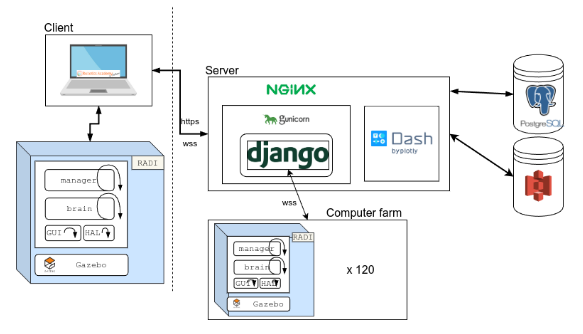
\includegraphics[width=9cm, keepaspectratio]{img/arquitectura.png}
  \caption{Estructura de Unibotics.}\label{fig:arquitectura}
\end{figure}

La base de datos de Unibotics está organizada para almacenar toda la información necesaria para el funcionamiento de la plataforma, desde los datos de los usuarios hasta los resultados de las simulaciones. Aunque toda esta información se encuentra en una única base de datos, está organizada en diferentes tablas que cubren varias áreas clave de la plataforma.

Por ejemplo, la información relacionada con los ejercicios y los universos de simulación está almacenada en tablas como exercises y exercise\_universes, las cuales permiten asociar ejercicios a los distintos entornos de simulación disponibles. Esto asegura que un mismo ejercicio pueda ejecutarse en varios universos, proporcionando flexibilidad en las simulaciones.

También está la información sobre los robots y los mundos de simulación, que se guarda en tablas como robots y worlds. Estas tablas contienen detalles sobre la configuración de los robots y los mundos de simulación, lo que permite a la plataforma gestionar los recursos necesarios para ejecutar los ejercicios en el entorno correcto.

Por otro lado, las tablas de logs, como log\_session y log\_exercises, almacenan los registros más importantes sobre la actividad de los usuarios. Estos logs incluyen información detallada sobre la duración de las sesiones de los usuarios, los ejercicios realizados y las fechas en las que se realizaron. Estos datos son fundamentales para generar los dashboards y análisis sobre el comportamiento de los usuarios en la plataforma.

Además, la base de datos gestiona también los datos clave sobre los usuarios, los permisos de acceso y las máquinas de granja (contenedores Docker) que ejecutan los ejercicios. Aquí se guardan los detalles de los usuarios y cómo se relacionan con los ejercicios a los que tienen acceso, así como el estado de las máquinas que se utilizan para ejecutar los ejercicios.

En la Figura \ref{fig:ER}, se muestra el diagrama de entidad-relación (ER) que ilustra cómo todas estas tablas están conectadas entre sí y cómo se organiza la información en la base de datos. Este diagrama es esencial para comprender cómo fluye la información dentro del sistema y cómo se gestionan las relaciones entre los diferentes elementos.

\begin{figure}[H]
    \centering
    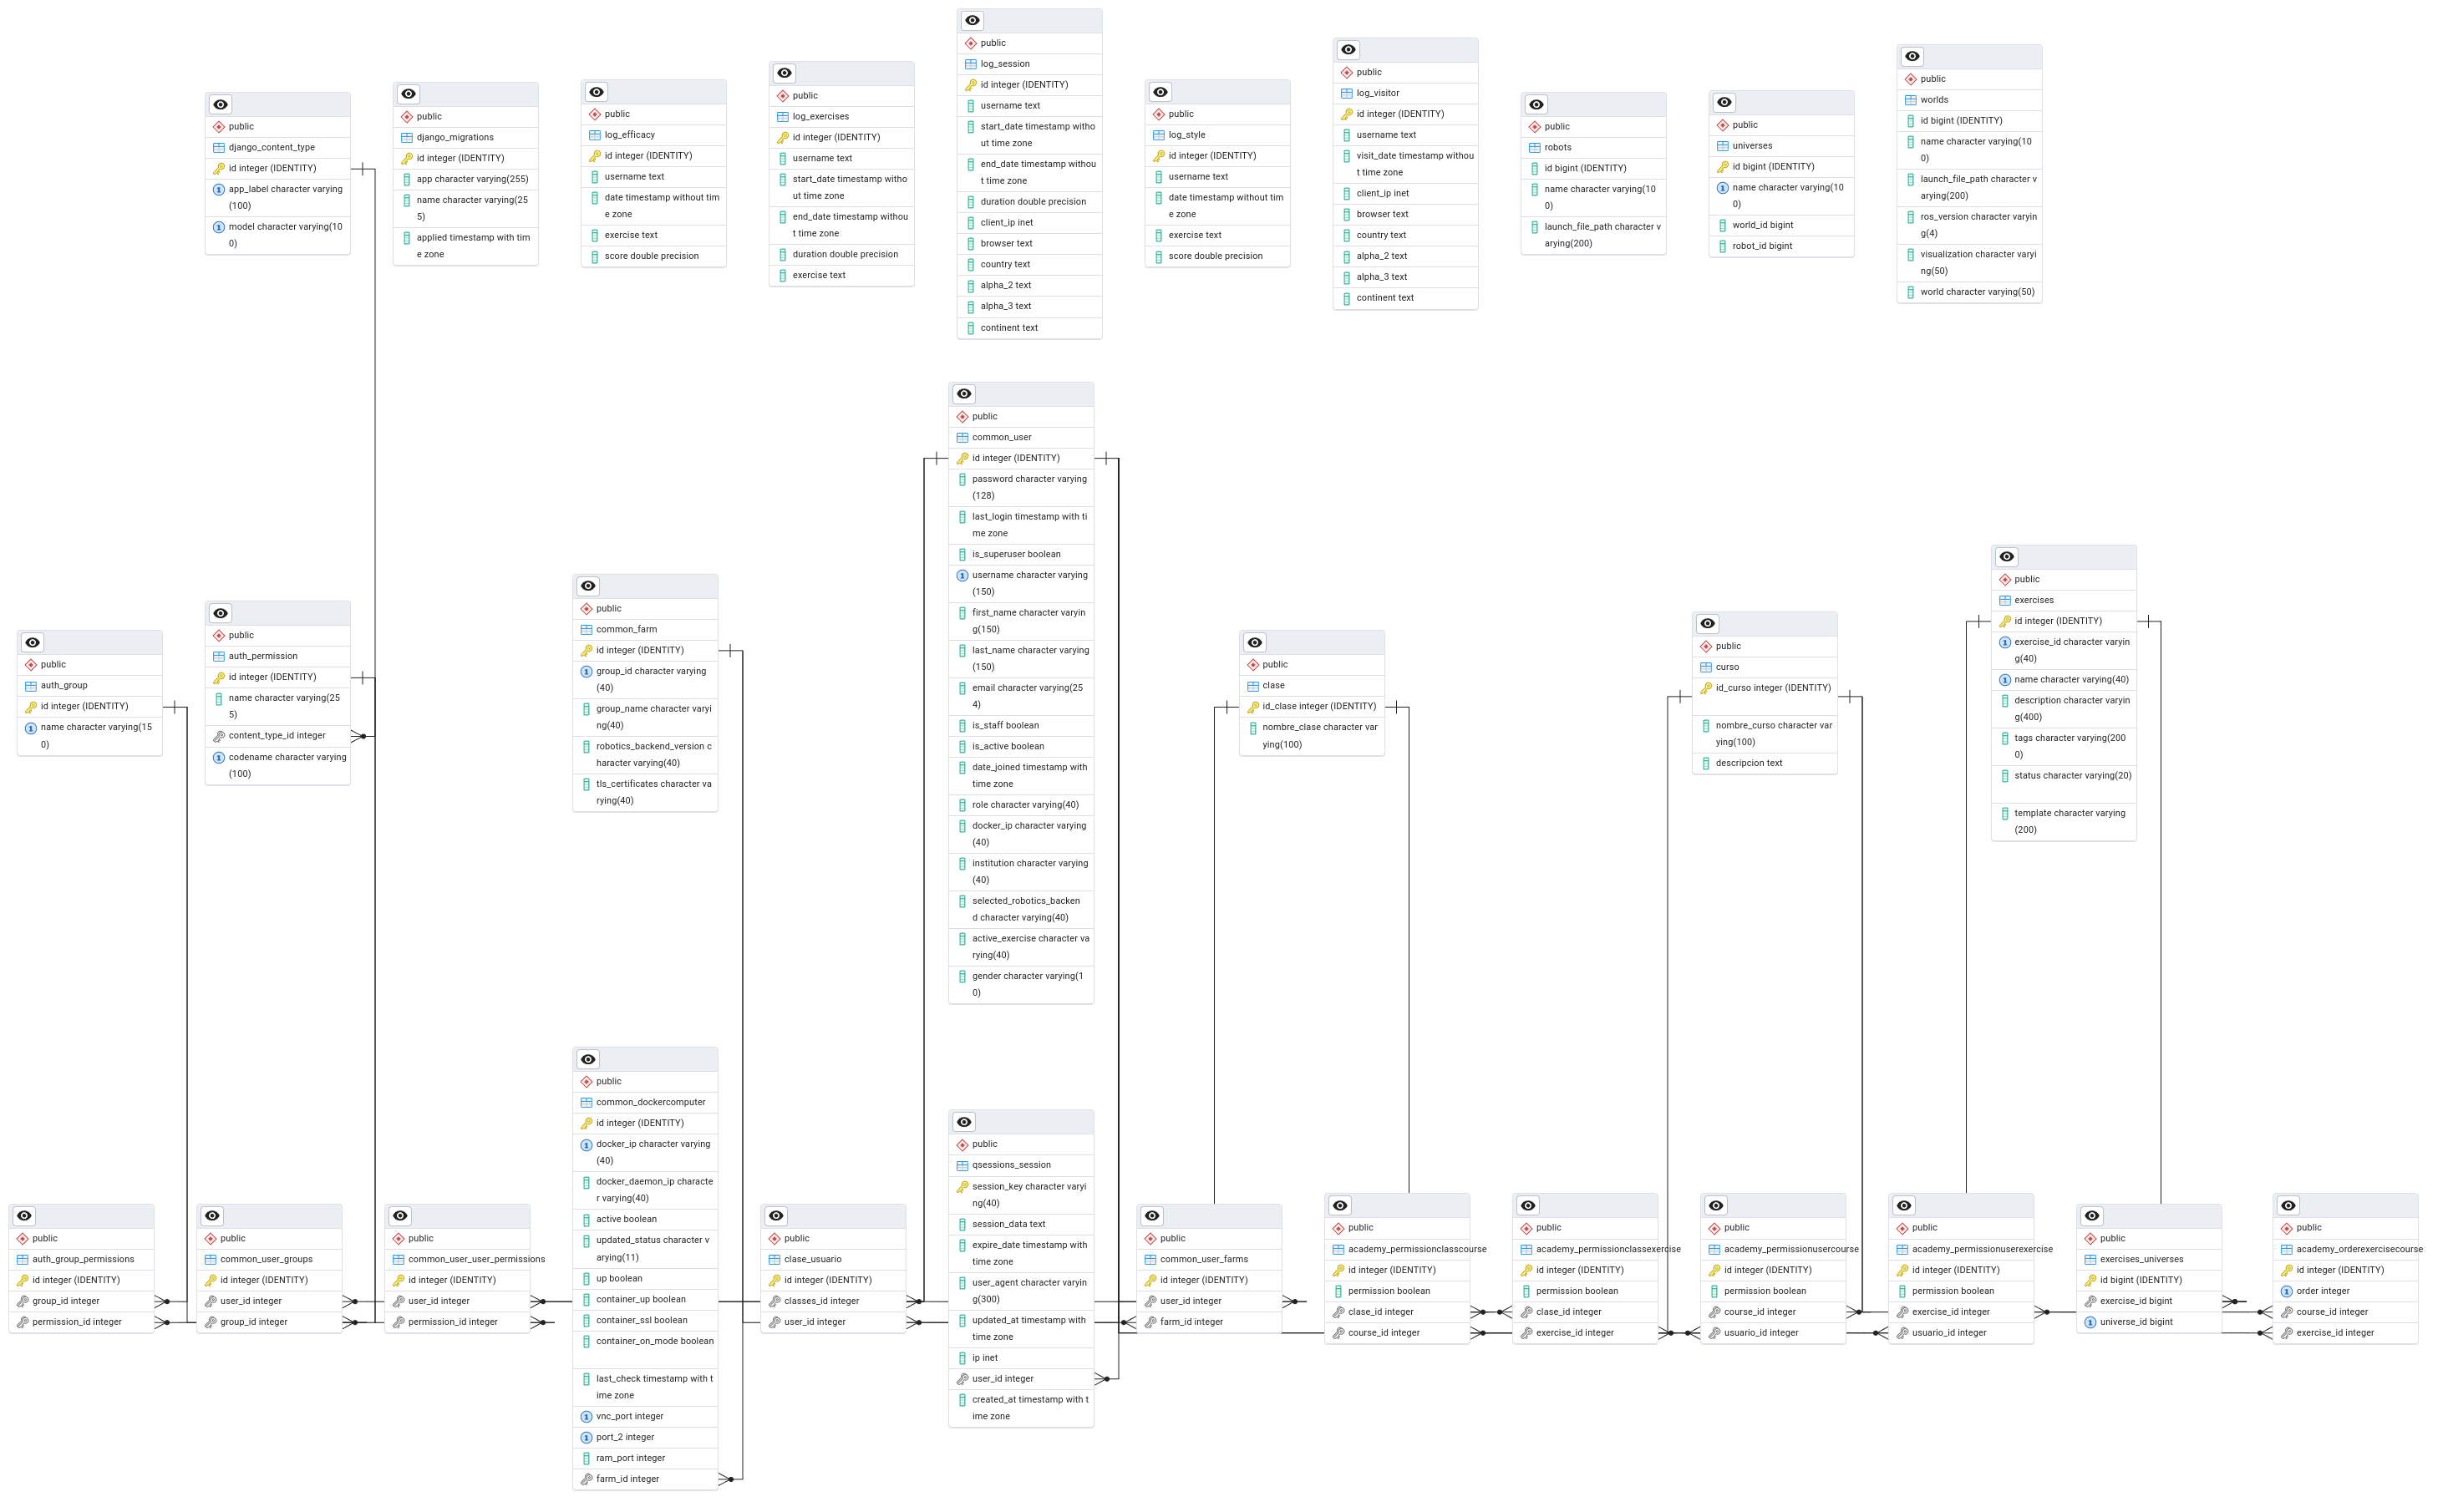
\includegraphics[angle=90, width=\textwidth, height=\textheight, keepaspectratio]{img/ER.png}
    \caption{Diagrama entidad-relación.}
    \label{fig:ER}
\end{figure}


Finalmente, en el apendice A \ref{chap:apendiceA}, encontrarás ejemplos de consultas SQL que te permitirán obtener información directamente de las tablas de logs y realizar análisis sobre la actividad de los usuarios y su interacción con los ejercicios.

\section{Despliegue Local en Linux}

Para poder probar y depurar todos los componentes de Unibotics de forma sencilla, instalé un entorno completo en mi máquina Linux (despliegue “D1”). En primer lugar, creé un entorno virtual de Python 3.8 para aislar las dependencias del proyecto sin afectar al sistema. A continuación, cloné el repositorio de \texttt{unibotics-webserver} junto con sus submódulos y ejecuté la instalación de los paquetes necesarios desde el fichero \texttt{utils/requirements.txt}.  

Dado que Unibotics utiliza PostgreSQL como base de datos, levanté un contenedor Docker con esa imagen. Esto me permitió iniciar, detener o reiniciar la base de datos con total comodidad y sin instalar nada en el sistema. Tras arrancar el contenedor, apliqué los dumps de Robotics Infrastructure y Robotics Academy para cargar los universos y ejercicios, ejecuté las migraciones de Django para crear el resto de tablas y, finalmente, importé datos de prueba de cursos pasados para disponer de una muestra amplia sobre la que trabajar.

En la parte de frontend, configuré los enlaces simbólicos que Webpack necesita para localizar los componentes de RoboticsAcademy, instalé las dependencias de Node y arrancé el modo desarrollo de Webpack. Con ello, cualquier cambio en el código React se recompila al vuelo y se refleja en el navegador.

Con este entorno ya puedo levantar la plataforma completa en local, probar cada cambio y comprobar al instante cómo funciona sin miedo a romper nada en producción. Esto me proporciona una zona de pruebas segura donde experimentar libremente y acelerar el ciclo de desarrollo y depuración.


\cleardoublepage

%%%%%%%%%%%%%%%%%%%%%%%%%%%%%%%%%%%%%%%%%%%%%%%%%%%%%%%%%%%%%%%%%%%%%%%%%%%%%%%%

%%%%%%%%%%%%%%%%%%%%%%%%%%%%%%%%%%%%%%%%%%%%%%%%%%%%%%%%%%%%%%%%%%%%%%%%%%%%%%%%
% EXPERIMENTOS Y VALIDACIÓN %
%%%%%%%%%%%%%%%%%%%%%%%%%%%%%%%%%%%%%%%%%%%%%%%%%%%%%%%%%%%%%%%%%%%%%%%%%%%%%%%%

\chapter{Experimentos y validación}
\label{chap:experimentos}

En esta sección expondré los distintos dashboards que he desarrollado con el objetivo de poder visualizar y analizar la información que está almacenada en la base de datos de Unibotics.

Cada dashboard se centra en distintas características del comportamiento del usuario, para su desarrollo he utilizado el framework Dash de Python junto con Plotly para la visualización gráfica y la información se extrae directamente desde la base de datos PostgreSQL mediante consultas SQL específicas.

En los siguientes apartados expondré de forma individual cada uno de los dashboard desarrollados, explicando su propósito, los datos que representa, el porqué ese tipo de visualización y las diferentes conclusiones que pueden obtenerse sobre el comportamiento de los usuarios.

A continuación, se presentan las tablas SQL de las que se extrae la información utilizada en los dashboards.

\begin{table}[H]
\centering
\caption*{\textbf{Tabla 4.1} \\
\textit{Tablas SQL utilizadas de la base de datos de Unibotics.}}
\begin{tabular}{lp{10cm}}
\toprule
\textbf{Tabla} & \textbf{Descripción} \\
\midrule
Log\_session & Contiene información sobre las sesiones iniciadas por los usuarios. Entre los campos más relevantes se encuentran el nombre del usuario, la fecha y hora de inicio de la sesión, la duración total en segundos y el país desde el cual se conecta el usuario. \\
Log\_exercises & Contiene información sobre los accesos de los usuarios a los distintos ejercicios disponibles. Entre los campos más relevantes se encuentran el nombre del usuario, el nombre del ejercicio al que accede, la duración de la interacción, la fecha y hora de inicio, así como otros datos relacionados con la actividad. \\
Common\_user & Reúne información general sobre los usuarios registrados en la plataforma. Aunque cuenta con múltiples campos, el más relevante para este trabajo es el género del usuario. \\
Exercises & Contiene un listado con los distintos ejercicios disponibles en la plataforma \\
\bottomrule
\end{tabular}
\vspace{1ex}

\begin{flushleft}
\textit{Nota.} La base de datos de Unibotics contiene mas tablas como vimos en \ref{sec:arquitectura}, pero estas son las que uso para realizar los Dashboards.
\end{flushleft}
\end{table}




\section{DASHBOARD 1A}

El Dashboard 1A nos permite analizar la duración total que un usuario ha dedicado a cada ejercicio de la plataforma.

Para poder obtener la información de duración por ejercicio, el dashboard se conecta directamente a la base de datos PostgreSQL de Unibotics mencionada anteriormente.
Una vez establecida la conexión, la aplicación Dash ejecuta una consulta SQL parametrizada con el nombre de usuario introducido en el input.

La consulta SQL aprovecha la funcionalidad de agrupación y agregación de SQL: se filtran los registros por el usuario seleccionado y luego se agrupan por el identificador de ejercicio, calculando la suma de todos los tiempos asociados,la informacion se obtiene de la tabla log\_session. La consulta tiene esta forma:

aqui pego codigo sigp sin ser capaz no se porque no lo veo

De este modo, la propia consulta realiza el cálculo de la duración total (en segundos) acumulada para cada ejercicio realizado por el usuario indicado. La cláusula GROUP BY agrupa las filas que tienen el mismo valor de ejercicio y aplica la función agregada SUM() para sumar los datos de cada grupo.
En otras palabras, si el usuario ha realizado varias sesiones o intentos en un mismo ejercicio, todos esos tiempos se suman en un único resultado por ejercicio. Esta consulta retorna una tabla con dos columnas: el nombre de cada ejercicio y la suma de la duración total que el usuario ha invertido en él. Dichos resultados se cargan en un DataFrame de Pandas para su manipulación en la aplicación y posteriormente se emplean para generar la visualización.

\begin{figure}
  \centering
  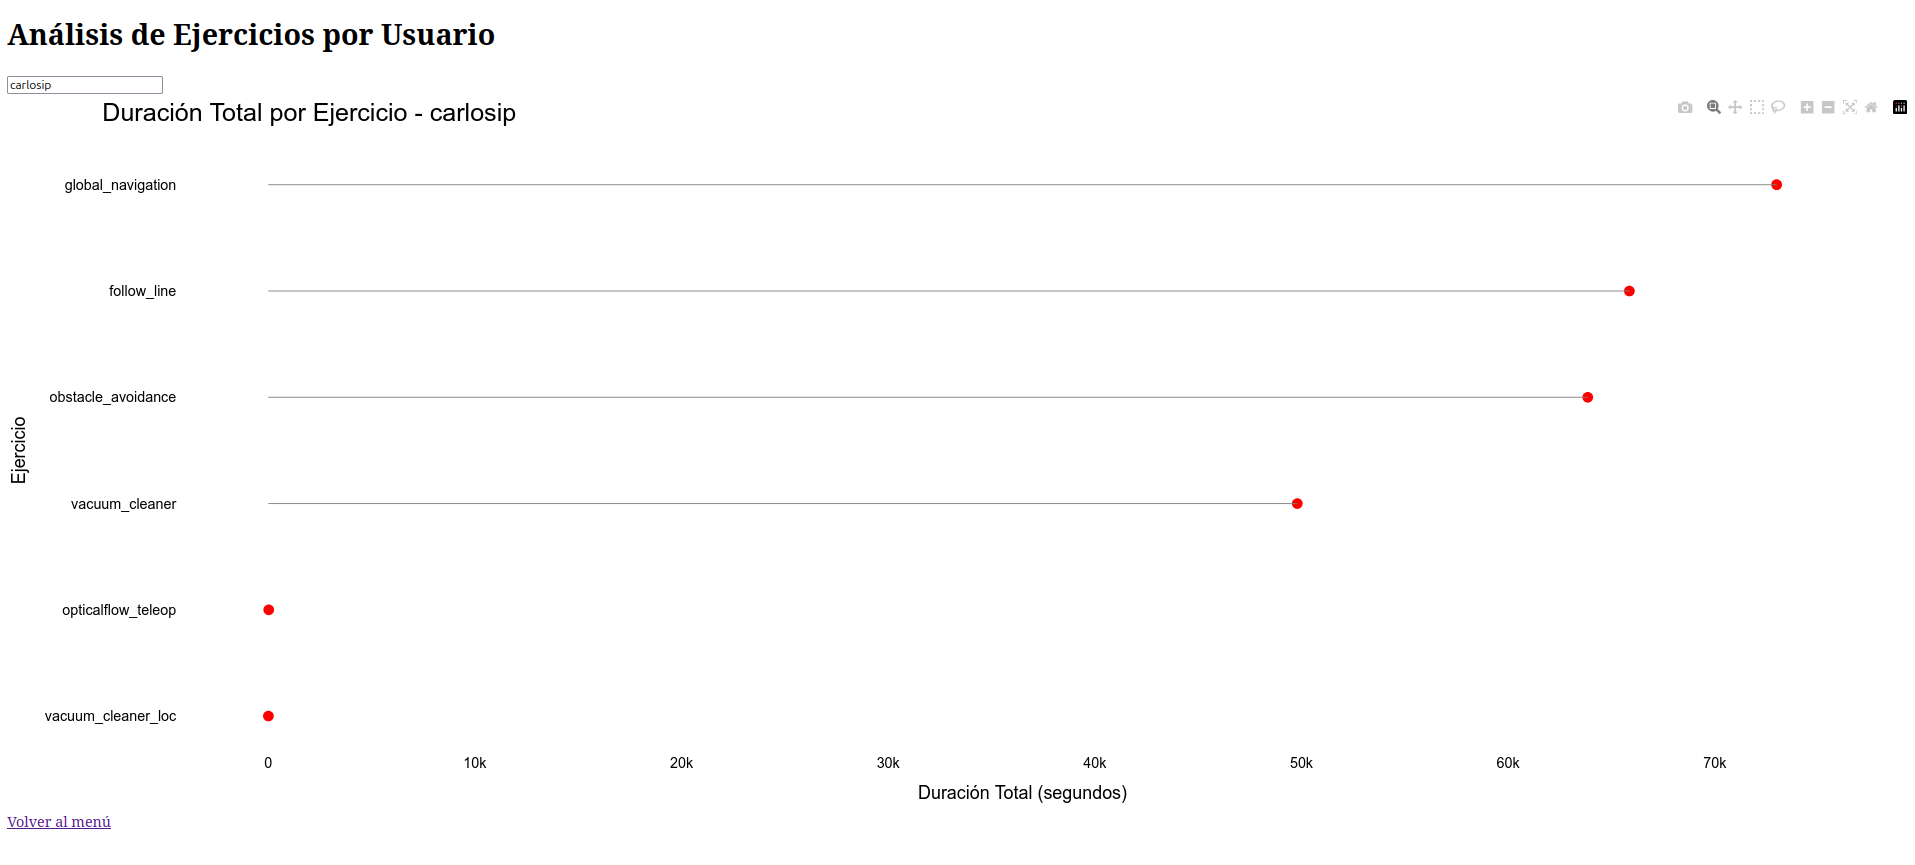
\includegraphics[width=9cm, keepaspectratio]{TFG/2024-tfg-alejandro-aguilera/memoria/img/1a.png}
  \caption{Dash 1a.}\label{fig:1a}
\end{figure}

Desde el punto de vista del usuario, el usuario ve un dashboard y un cuadro de texto donde poder escribir el nombre del usuario que deseas visualizar su duración total por ejercicio, una vez escrito un nombre de usuario carga el dashboard con la información de ese usuario.

El dashboard presenta los datos mediante un gráfico horizontal de líneas con puntos, también conocido como gráfico tipo lollipop. Este tipo de visualización es una variación de un diagrama de barras: la barra tradicional se transforma en una línea delgada y el valor se resalta con un marcador circular al final.

Explicar porque elegimos este tipo de gráfico (tambien importante que lo ordenamos de arriba a abajo porque era mejor visualmente)

La información presentada en el Dashboard 1A permite una rápida interpretación comparativa de la dedicación del usuario a los distintos ejercicios, gracias a ello podemos obtener varias conclusiones.

Identificación de ejercicios más y menos trabajados: Las longitudes de las líneas revelan de un vistazo cuáles son los ejercicios en los que el usuario ha invertido más tiempo y cuáles menos.

Detección de patrones de esfuerzo o dificultad: Una duración total muy elevada en cierto ejercicio podría indicar que el usuario tuvo dificultades significativas con ese ejercicio o que requirió múltiples intentos prolongados para completarlo,también podría significar que el ejercicio era muy extenso o el usuario dedicó tiempo extra explorando más allá de lo mínimo requerido. Por el contrario, ejercicios con duraciones muy bajas pueden sugerir que el usuario los completó rápidamente (quizá por ser sencillos o ya conocidos) o incluso que los abandonó pronto. En cualquier caso, los extremos en la distribución de tiempos señalan ejercicios que merecen una atención particular al evaluar el progreso del usuario.

Distribución del tiempo de aprendizaje: El conjunto de todas las duraciones permite ver cómo el usuario ha distribuido su tiempo de aprendizaje en la plataforma. Un perfil equilibrado mostraría barras (líneas) de duraciones relativamente similares entre ejercicios, mientras que un perfil más desequilibrado tendría unos pocos ejercicios dominando la mayor parte del tiempo total.

\section{DASHBOARD 1C}

Este dashboard tiene como objetivo mostrar la duración promedio de las sesiones de los usuarios de Unibotics, agrupadas por país. A través de un mapa mundial interactivo, se representa gráficamente qué países presentan una mayor o menor media de tiempo por sesión, permitiendo identificar patrones geográficos en el uso de la plataforma.

La información utilizada en este dashboard se obtiene desde la tabla log\_session,la consulta SQL utilizada agrupa los datos por país, calcula la suma total de duración y el número total de sesiones por país, y posteriormente se calcula en Python la duración promedio dividiendo ambos valores. La consulta tiene esta forma:

Aqui pego el codigo (pero nose como hacerlo bien)

A partir de esta consulta se genera un DataFrame de Pandas con el país y su respectiva duración promedio de sesión, que luego se utiliza para crear el gráfico. Este cálculo permite representar una métrica más equilibrada que la duración total (que podría estar sesgada por la cantidad de usuarios en un país), y proporciona una mejor medida de cómo interactúan los usuarios con la plataforma en promedio.

\begin{figure}
  \centering
  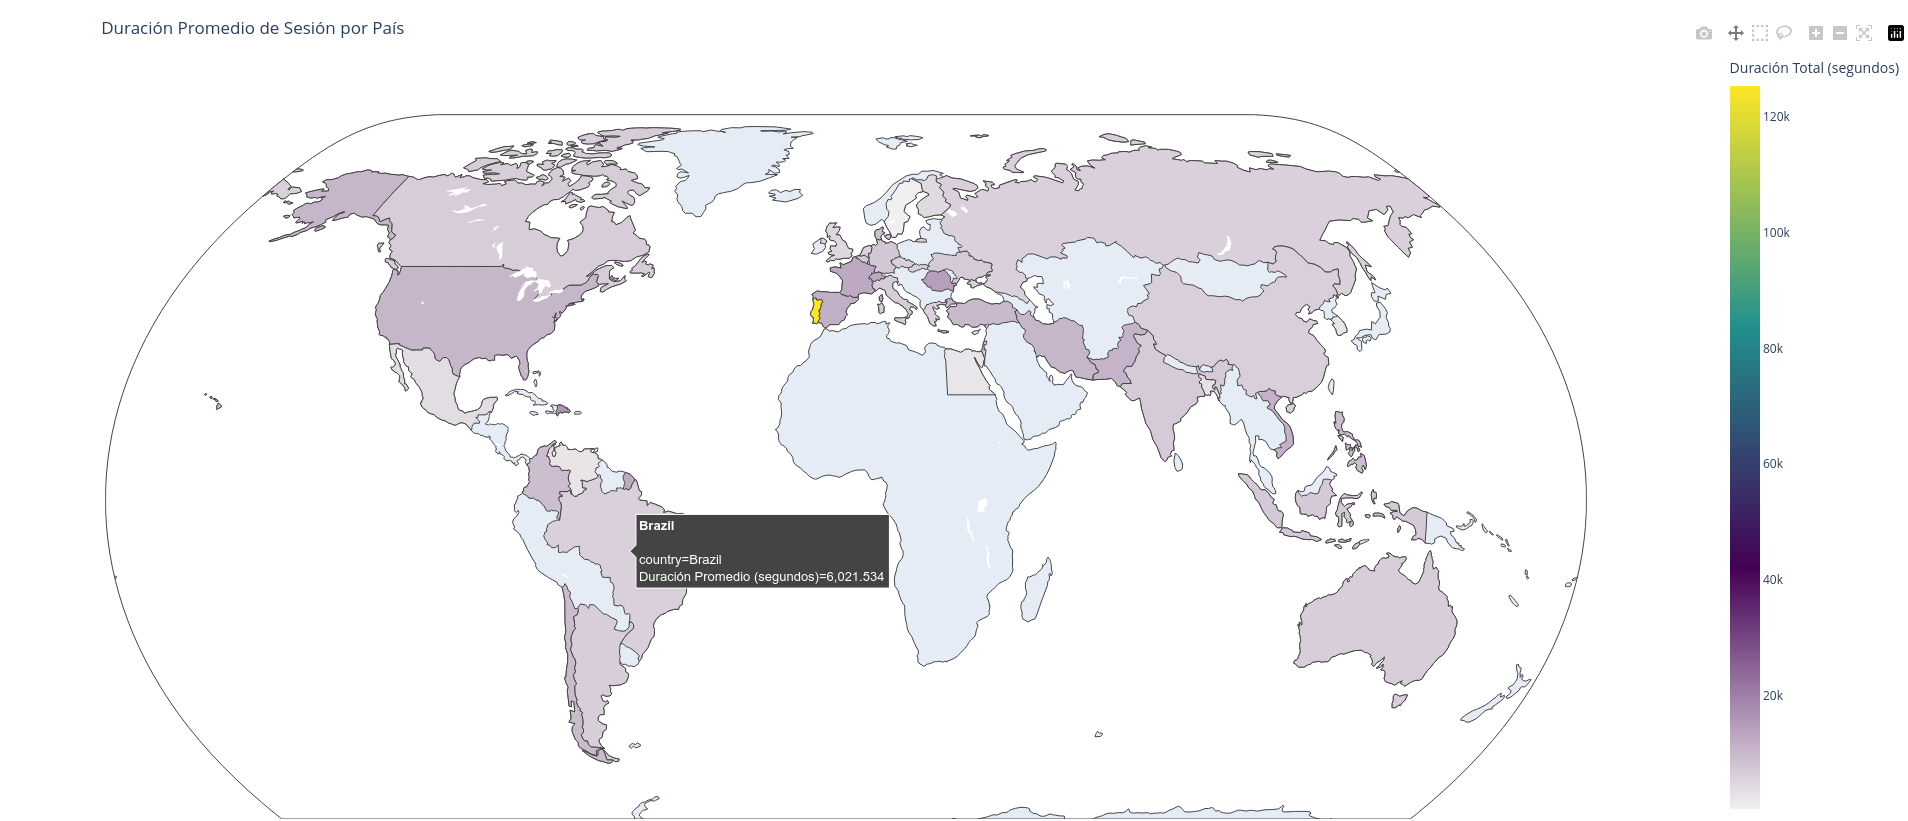
\includegraphics[width=9cm, keepaspectratio]{TFG/2024-tfg-alejandro-aguilera/memoria/img/1c.png}
  \caption{Dash 1c.}\label{fig:1c}
\end{figure}

El dashboard utiliza un mapa coroplético (choropleth map), generado mediante Plotly Express, en el que cada país se colorea en función de la duración promedio de sesión. Cuanto mayor es la duración, más intenso es el color asignado, siguiendo una escala cromática progresiva desde tonos claros hasta colores más saturados. En el ejemplo mostrado (foto anterior), se emplea una paleta de colores continua (aclarar que color dejo) personalizada para resaltar visualmente los valores extremos.

Explicar porque elegimos este tipo de gráfico

El dashboard ofrece información útil tanto a nivel técnico como estratégico.España aparece con una alta duración promedio, lo que sugiere un uso intensivo y posiblemente más prolongado por sesión, frente a países donde el uso puede ser más breve o esporádico.Sin embargo, países con bajas duraciones promedio pueden estar reflejando una adopción más reciente, una menor familiaridad con la plataforma o simplemente menor disponibilidad de tiempo por parte de los usuarios.

Desde el punto de vista de la administración de Unibotics, este dashboard puede ayudar a identificar mercados donde la plataforma tiene un mayor impacto o uso sostenido, lo cual puede influir en decisiones de soporte, localización de contenidos o expansión. Por el contrario, tambien puede ayudar a detectar regiones con bajo uso relativo, lo que puede motivar estrategias de difusión, colaboración educativa o mejora del acceso.

\section{DASHBOARD 2A}

Este dashboard tiene como objetivo mostrar la duración total acumulada de todas las sesiones de usuarios de Unibotics, agrupadas por país. A través de un mapa interactivo, permite observar en qué regiones geográficas se ha registrado un mayor tiempo de uso en conjunto, proporcionando una visión global de la distribución de la actividad en la plataforma.

La información utilizada en este dashboard se obtiene desde la tabla log\_session, la consulta SQL que se utiliza agrupa los datos por país y calcula la suma total de la duración de todas las sesiones correspondientes a cada país. La consulta tiene esta forma:

Aqui pego el codigo (pero nose como hacerlo bien)

A diferencia de otros dashboards que analizan promedios, en este caso se calcula simplemente la acumulación del tiempo total de uso de la plataforma por país. Esto permite identificar los países donde el uso absoluto de Unibotics ha sido más intenso.

Una vez obtenidos los resultados, se cargan en un DataFrame de Pandas con el pais y su respectiva duración total de sesiones y se utilizan como base para la representación gráfica en el mapa.

\begin{figure}
  \centering
  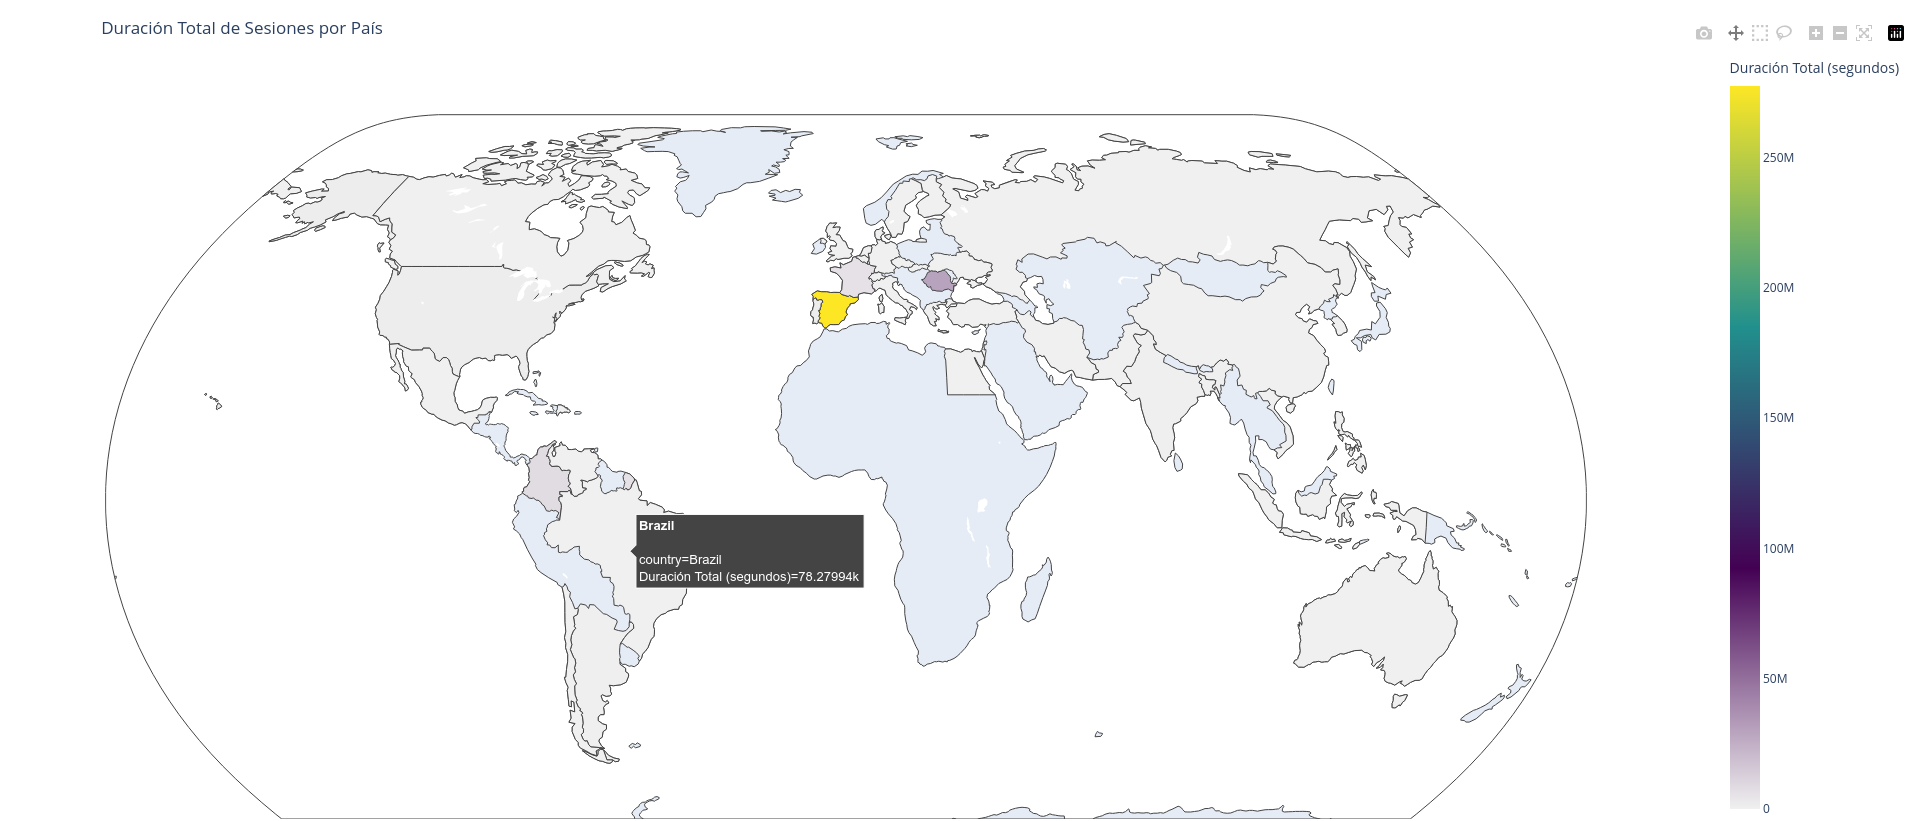
\includegraphics[width=9cm, keepaspectratio]{TFG/2024-tfg-alejandro-aguilera/memoria/img/2a.png}
  \caption{Dash 2a.}\label{fig:2a}
\end{figure}


El dashboard utiliza un mapa coroplético (choropleth map), generado mediante Plotly
Express, en el que cada país se colorea en función de la duración total de sesión. Cuan-
to mayor es la duración, más intenso es el color asignado, siguiendo una escala cromática
progresiva desde tonos claros hasta colores más saturados. En el ejemplo mostrado (foto
anterior), se emplea una paleta de colores continua (aclarar que color dejo) personalizada
para resaltar visualmente los valores extremos.

Explicar porque elegimos este tipo de gráfico

Del análisis del mapa (ver figura), se pueden obtener conclusiones como:

España destaca con el mayor volumen de tiempo total de sesiones, lo que refleja su fuerte implantación y uso intensivo de la plataforma, probablemente por ser el país de origen o principal mercado de Unibotics mientras que otros países europeos o latinoamericanos presentan niveles más bajos de duración acumulada, lo que puede interpretarse como una menor penetración o un uso más reciente de la plataforma en esas regiones.

Tambien se observan diferencias geográficas claras, algunos continentes como África o Asia presentan en general un uso más bajo, salvo excepciones, lo que podría señalar oportunidades de expansión o barreras de adopción actuales.

Desde el punto de vista de la gestión de Unibotics, este dashboard ayuda a ver en qué países la plataforma tiene más presencia. Esta información permite decidir mejor dónde hacer campañas, traducir contenidos o invertir en mejorar el servicio. Además, señala qué zonas podrían beneficiarse más de nuevas colaboraciones educativas

\section{DASHBOARD 2C}

Este dashboard muestra la evolución mensual del número de sesiones iniciadas en Unibotics a lo largo del año 2024, diferenciando también entre usuarios masculinos y femeninos. El objetivo es analizar cómo varía el uso de la plataforma mes a mes y si existen diferencias significativas por género.

Los datos provienen de las tablas log\_session y common\_user,la consulta SQL utilizada realiza una agregación mensual,teniendo en cuenta: el total de sesiones iniciadas en cada mes,el número de sesiones realizadas por usuarias (género femenino)y el número de sesiones realizadas por usuarios (género masculino).
La consulta tiene esta forma:

Aqui pego el codigo (pero nose como hacerlo bien)

Una vez extraídos, los datos se procesan en Pandas para asegurarse de que los meses estén correctamente ordenados de enero a diciembre, y se formatea el nombre de los meses.


\begin{figure}
  \centering
  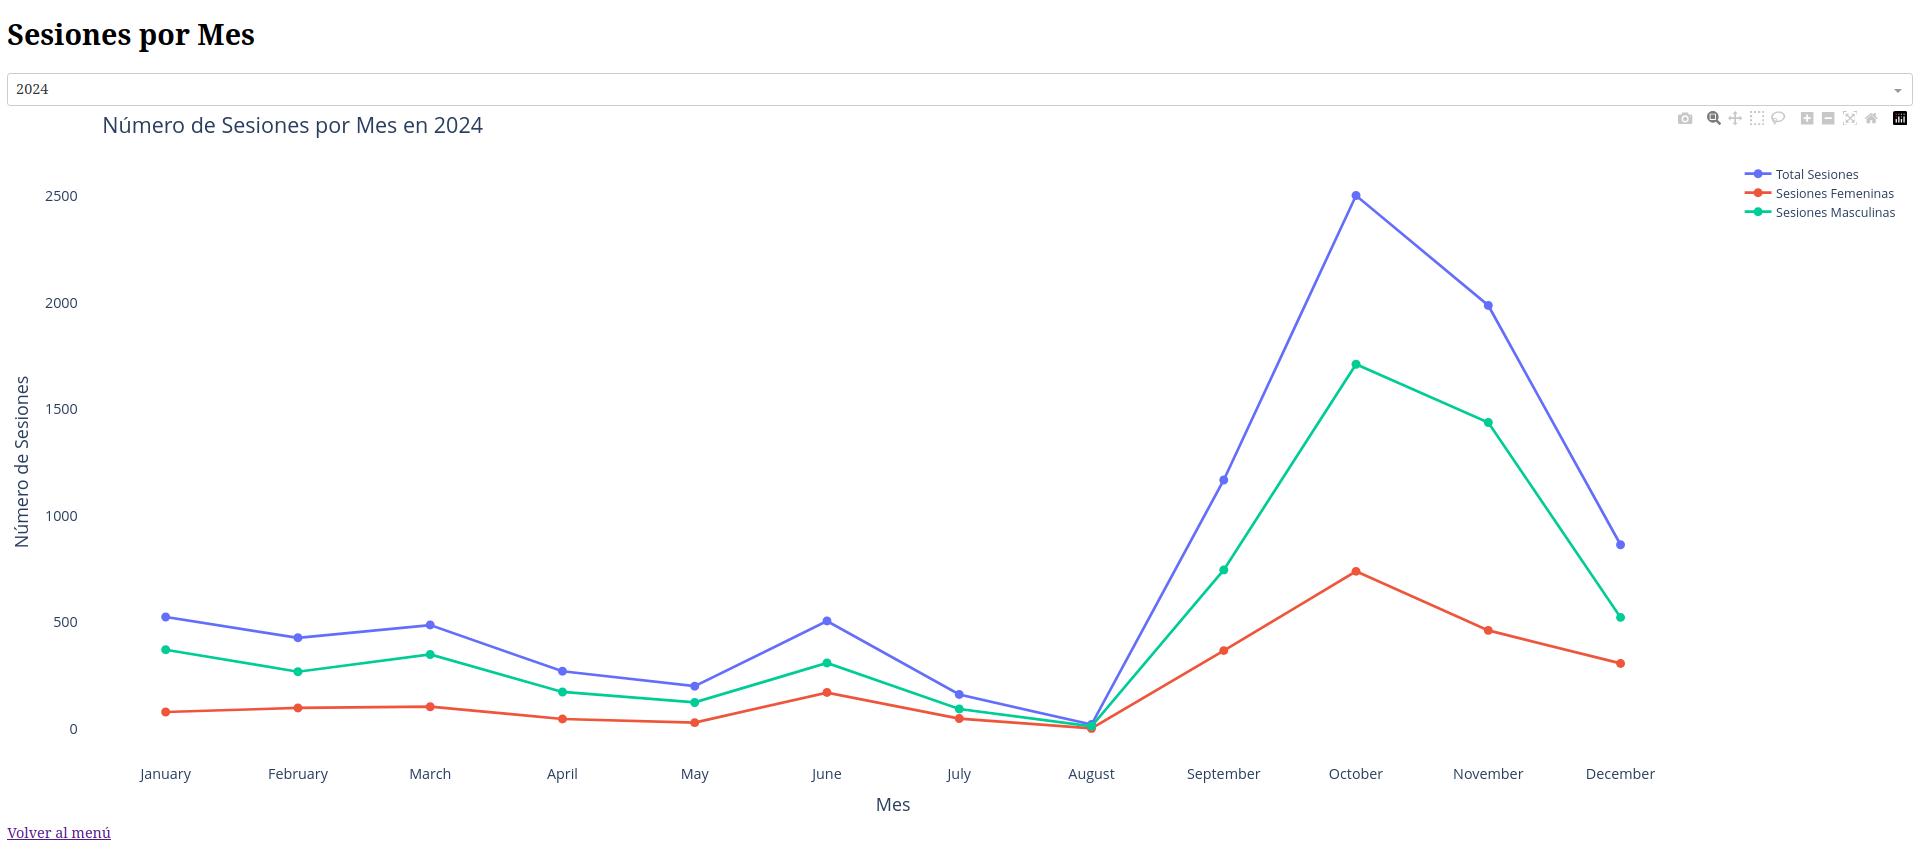
\includegraphics[width=9cm, keepaspectratio]{TFG/2024-tfg-alejandro-aguilera/memoria/img/2c.png}
  \caption{Dash 2c.}\label{fig:2c}
\end{figure}
El dashboard utiliza un gráfico de líneas para representar la evolución de las sesiones durante el año. Se incluyen tres líneas:

    Total de sesiones (en azul).
    Sesiones femeninas (en rojo).
    Sesiones masculinas (en verde).

Cada punto en el gráfico representa el número de sesiones registradas en ese mes para cada categoría.

Explicar porque elegimos este tipo de gráfico

Explicar conclusiones porque de aqui mas alla de que en verano nadie hace nada no se que mas decir.


\section{DASHBOARD 3A}

Este dashboard analiza cómo se distribuyen los usuarios de Unibotics según el tiempo total que han dedicado a un ejercicio específico. Utiliza una escala logarítmica para poder representar mejor las diferencias en las duraciones, que pueden ser muy grandes entre unos usuarios y otros.

Los datos provienen de las tablas log\_exercises y exercises.El usuario ve un desplagable de ejercicios que permite seleccionar un ejercicio concreto mediante un desplegable. Una vez seleccionado, se ejecuta una consulta SQL que suma el tiempo total que cada usuario ha dedicado a ese ejercicio.
La consulta tiene esta forma:

Aqui pego el codigo (pero nose como hacerlo bien)

Después de obtener los datos, se aplica una transformación logarítmica al valor de duración total. Esto se hace para reducir la dispersión de los datos: como hay usuarios que pueden haber pasado desde unos pocos segundos hasta varias horas en un mismo ejercicio, el uso de una escala logarítmica permite ver toda la distribución de una forma más equilibrada.

\begin{figure}
  \centering
  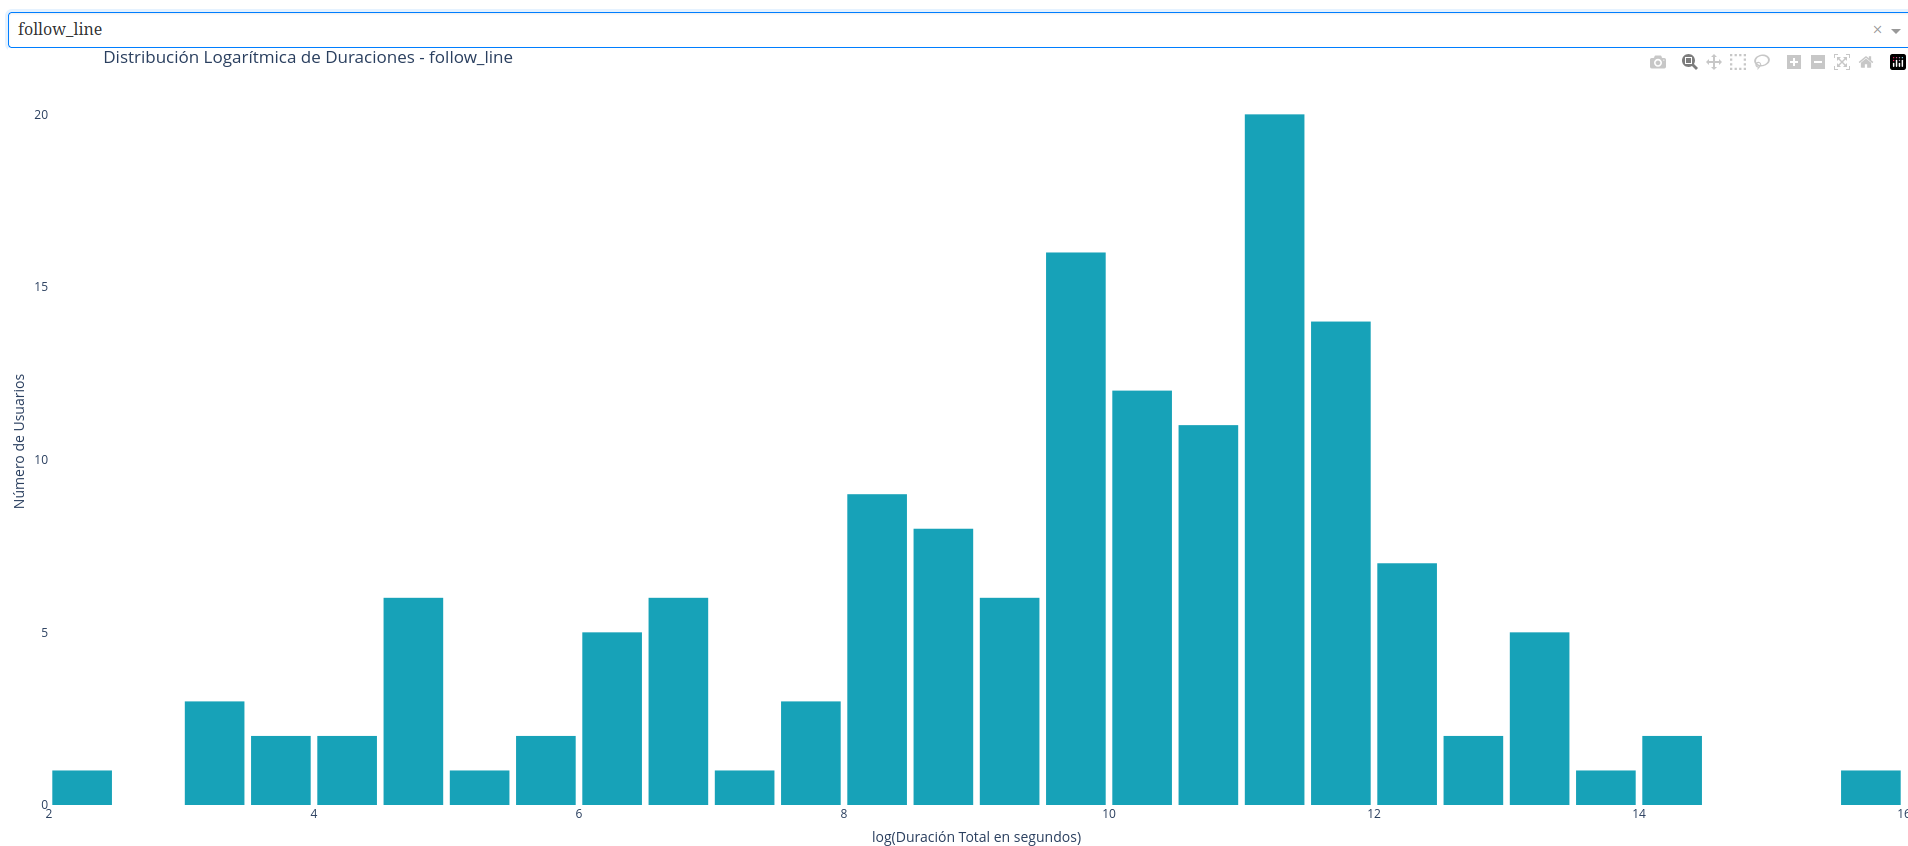
\includegraphics[width=9cm, keepaspectratio]{TFG/2024-tfg-alejandro-aguilera/memoria/img/3a.png}
  \caption{Dash 3a.}\label{fig:3a}
\end{figure}

El dashboard muestra los datos en un histograma, donde el eje horizontal representa el logaritmo de la duración total (en segundos) y el eje vertical representa el número de usuarios que tienen una duración dentro de cada rango.

Cada barra del histograma muestra cuántos usuarios cayeron en ese rango de duraciones. La escala logarítmica en el eje X permite visualizar mejor los datos, ya que de otra manera la mayoría de los usuarios quedarían agrupados en duraciones bajas y sería difícil distinguir diferencias.

Explicar porque elegimos este tipo de gráfico

El análisis del histograma permite entender cómo se comportan los usuarios al realizar un determinado ejercicio. Al observar la distribución de los tiempos, podemos ver si la mayoría de los usuarios completan el ejercicio en un tiempo parecido o si existen grandes diferencias entre ellos. 

Cuando los tiempos se agrupan principalmente en valores bajos, suele indicar que el ejercicio es sencillo o que muchos usuarios no llegaron a dedicarle demasiado tiempo, quizás porque lo abandonaron pronto. En cambio, cuando hay una gran variedad de tiempos, podemos interpretar que el ejercicio tiene un nivel de dificultad más variable o que, por su diseño, permite a los usuarios dedicarle más tiempo explorando distintas soluciones. 

Para los profesores, ofrece una forma de detectar si el ejercicio está bien equilibrado en cuanto a dificultad, o si sería necesario ajustarlo para mejorar la experiencia de aprendizaje.

\section{DASHBOARD 3B}

Este dashboard muestra cómo se distribuye el tiempo que cada usuario ha dedicado a distintos ejercicios de Unibotics. Utiliza diagramas de caja (boxplots) aplicando una escala logarítmica para representar mejor las diferencias entre los usuarios.

Los datos se obtienen de la tabla log\_exercises. Se agrupa la información por nombre de ejercicio y por usuario, sumando la duración total que cada uno ha dedicado a cada ejercicio. Solo se consideran aquellos casos donde el tiempo total registrado es mayor que cero.
La consulta tiene esta forma:

Aqui pego el codigo (pero nose como hacerlo bien)

Una vez extraídos los datos, se calcula el logaritmo de la duración total para cada usuario. Esto se hace para normalizar los valores, ya que algunos usuarios pueden tener tiempos muy pequeños y otros muy grandes, y la escala logarítmica ayuda a visualizar mejor esa variabilidad.

\begin{figure}
  \centering
  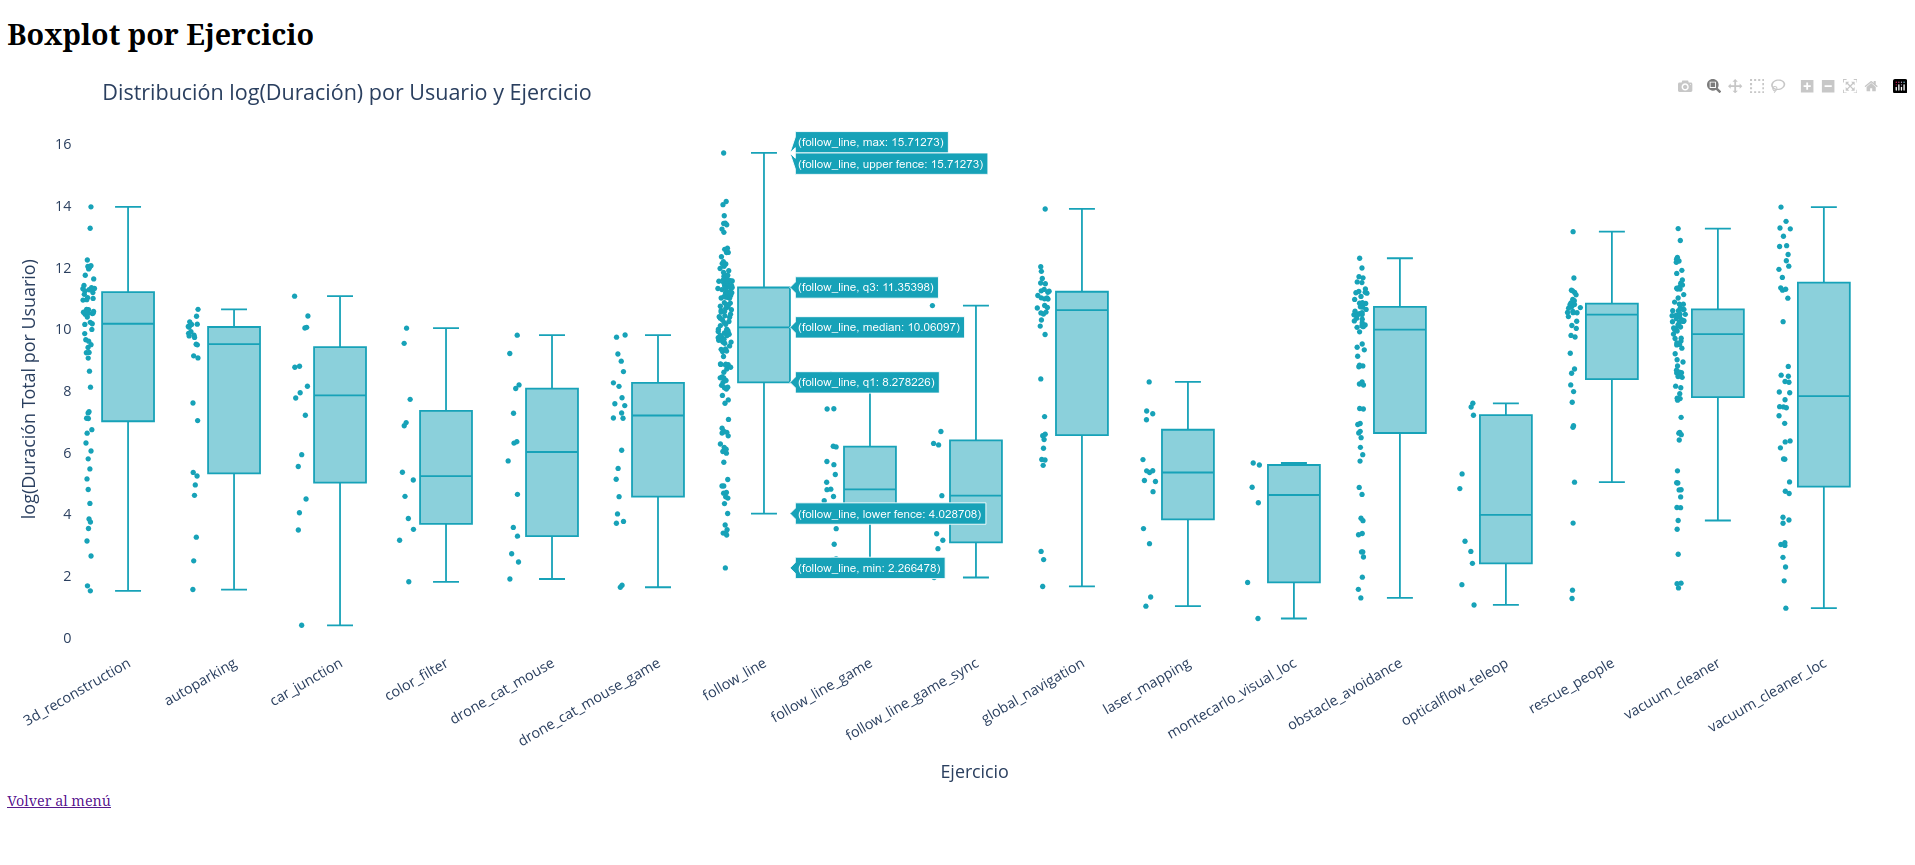
\includegraphics[width=9cm, keepaspectratio]{TFG/2024-tfg-alejandro-aguilera/memoria/img/3bb.png}
  \caption{Dash 3b.}\label{fig:3b}
\end{figure}

Cada ejercicio se representa en el eje horizontal, mientras que en el eje vertical se muestra el logaritmo del tiempo total invertido por los usuarios. Para cada ejercicio, el boxplot muestra:

La mediana de las duraciones (línea central del rectángulo).
El rango intercuartílico (el ancho de la caja), que representa la mayoría de los usuarios.
Los valores extremos o atípicos (puntos dispersos fuera de la caja).

Gracias a este tipo de gráfico es posible visualizar de forma clara cómo varía la dedicación de los usuarios en cada ejercicio, y detectar si hay muchos usuarios que dedican tiempos muy distintos o si la mayoría se concentra en valores similares. Además, se muestran todos los puntos individuales sobre los diagramas, lo que permite ver mejor la dispersión real de los datos.

Este dashboard permite comparar de manera rápida cómo se comportan los usuarios en cada ejercicio. Se puede ver si la mayoría de los alumnos dedican un tiempo similar o si hay mucha diferencia entre unos y otros. También ayuda a detectar ejercicios en los que algunos usuarios invierten mucho más tiempo, lo que podría significar que son más complicados o que resultan especialmente interesantes. Además, permite identificar actividades donde hay muchos casos extremos, lo que podría indicar que el ejercicio no está bien planteado o que su dificultad varía demasiado entre estudiantes. Para los profesores, esta información es útil para saber qué ejercicios podrían necesitar cambios o mejoras, y para entender mejor cómo se enfrentan los alumnos a las tareas. Para quienes diseñan los contenidos, el análisis sirve para ver si los ejercicios provocan el tipo de trabajo esperado o si sería buena idea añadir ayudas o dividir las actividades.

\section{DASHBOARD 3C}

Este dashboard es muy similar al anterior (Dashboard 3B), ya que también utiliza diagramas de caja (boxplots) para representar los datos, pero con una diferencia importante: en lugar de analizar el tiempo total que cada usuario dedica a un ejercicio, aquí se analiza la duración de cada sesión individual.

Mientras que en el 3B (esto lo cambiare cuando esten todos) sumábamos todas las sesiones de un usuario para un ejercicio determinado, en este dashboard se estudia cada sesión por separado, sin agruparlas. Además, también se aplica una escala logarítmica para representar mejor las diferencias en los tiempos, ya que algunas sesiones pueden durar solo unos pocos segundos y otras mucho más.

Para obtener estos datos se utiliza una consulta SQL sencilla que selecciona, para cada registro de sesión, el nombre del ejercicio y la duración de esa sesión concreta:

aqui pongo el codigo

\begin{figure}
  \centering
  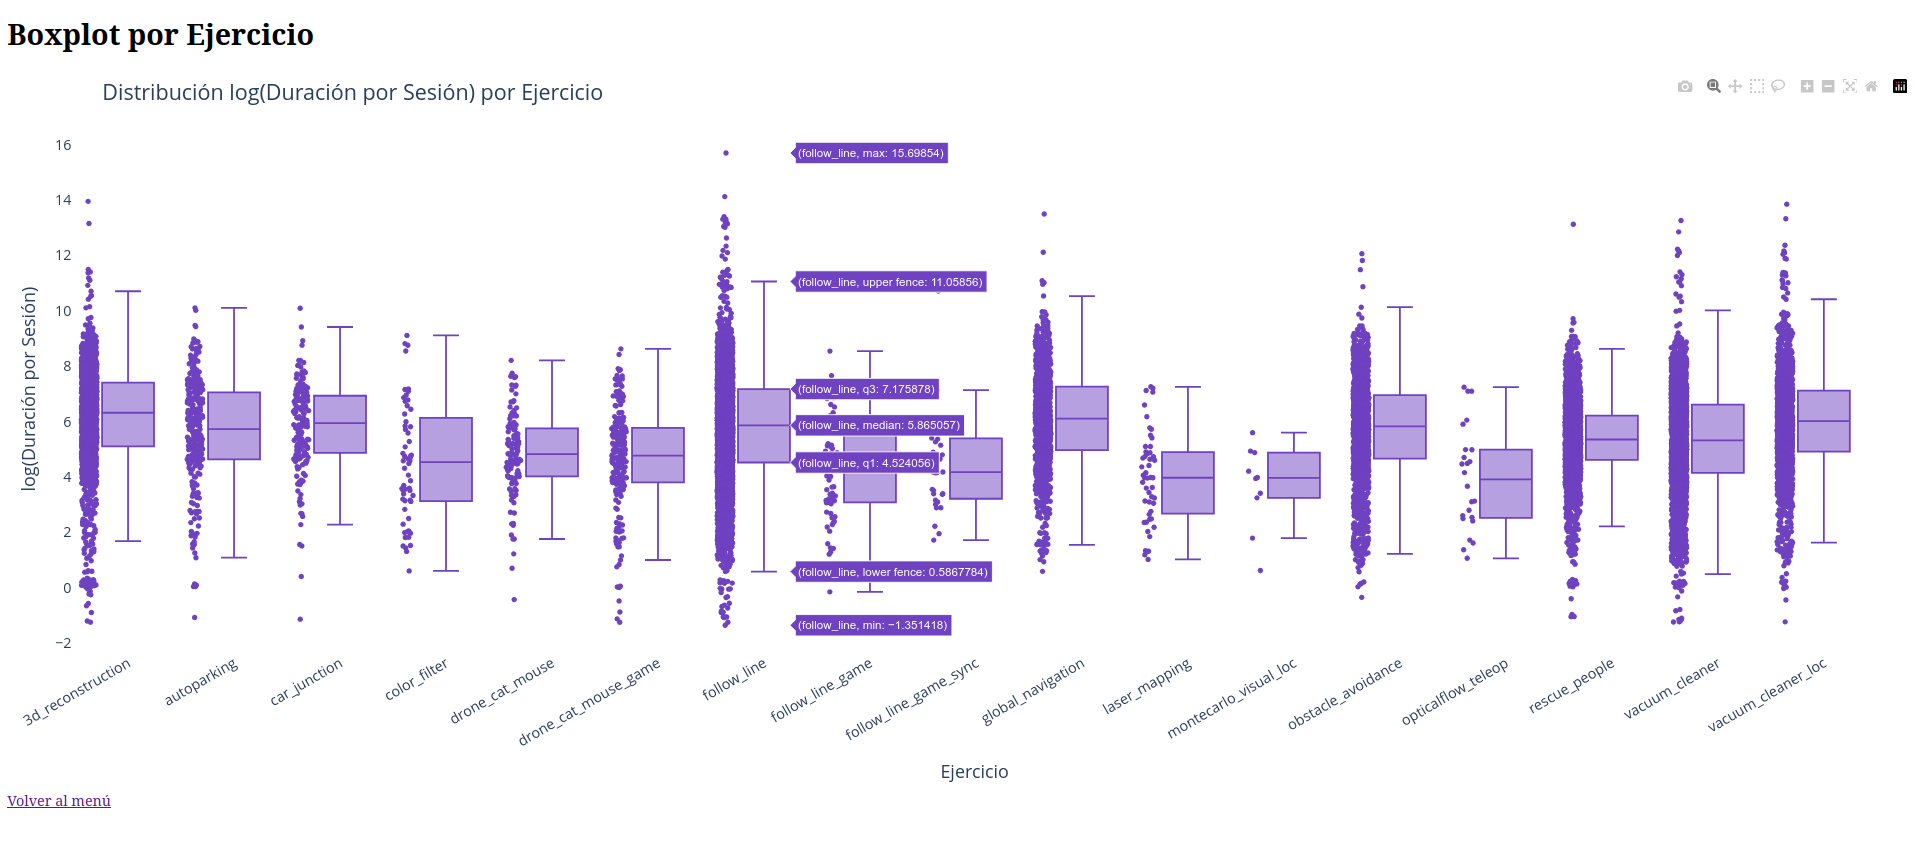
\includegraphics[width=9cm, keepaspectratio]{TFG/2024-tfg-alejandro-aguilera/memoria/img/3c.png}
  \caption{Dash 3c.}\label{fig:3c}
\end{figure}

El objetivo de este dashboard es ofrecer una visión más detallada sobre cómo varía el tiempo de trabajo en cada intento o sesión concreta, algo que no era visible en el Dashboard 3B, donde sólo veíamos el esfuerzo acumulado de cada usuario. Aquí podemos detectar, por ejemplo, si un ejercicio tiene sesiones generalmente cortas o si hay mucha variación entre los intentos de los distintos usuarios.

Esta representación es útil para entender mejor el comportamiento real dentro de cada ejercicio: permite ver si los estudiantes tienden a resolver los ejercicios de forma rápida o si, por el contrario, dedican mucho tiempo en intentos sucesivos. Además, puede ayudar a detectar ejercicios que generan más dispersión en el tiempo por sesión, lo que puede ser una pista sobre su dificultad o sobre la necesidad de mejorar su planteamiento o las instrucciones dadas.

\section{como poner codigo}


Es bastante habitual que se reproduzcan fragmentos de código en la memoria de un TFG/TFM.
Esto permite explicar detalladamente partes del desarrollo que se ha realizado que se consideren
de especial interés. No obstante, tampoco es conveniente pasarse e incluir demasiado código en
la memoria, puesto que se puede alargar mucho el documento. Un recurso muy habitual es subir
todo el código a un repositorio de un servicio de control de versiones como GitHub o GitLab,
y luego incluir en la memoria la URL que enlace a dicho repositorio.





Para incluir fragmentos de código en un documento \LaTeX se pueden combinar varias
herramientas:

\begin{itemize}
    \item El entorno \mintinline{latex}{\begin{listing}[]...\end{listing}} permite crear
    un marco en el que situar el fragmento de código (parecido al generado cuando insertamos
    una tabla o una figura). Podemos insertar también una descripción (\textit{caption})
    y una etiqueta para referenciarlo luego en el texto.
    
    \item Dentro de este entorno, se puede utilizar el paquete 
    \mintinline{latex}{minted}~\footnote{\url{https://es.overleaf.com/learn/latex/Code_Highlighting_with_minted}},
    que utiliza el paquete Python Pygments para resaltado de sintaxis (coloreando el
    código). Como se puede ver en el siguiente ejemplo, hay muchas opciones de configuración
    que permiten controlar cómo se va a mostrar el código (incluir números de línea, saltos
    de línea, tamaño y tipo de fuente, espaciado, código de colores para resaltado, etc.).
\end{itemize}

\begin{listing}[h!]
    \caption{Lectura de un fichero *.csv y tipado de datos.}{}
    \label{lst:1}
    \begin{minted}[breaklines, fontsize=\footnotesize, baselinestretch=1]{python}
# A dictionary is built to define the data type contained by each column
dtype_scheme ={'budget': np.int64, 'genres': np.object, 'homepage': np.str, 'id': np.int64, 'keywords': np.object, 'original_language': np.str, 'original_title': np.str, 'overview': np.str, 'popularity': np.float64, 'production_companies': np.object, 'production_countries': np.object, 'release_date': np.object, 'revenue': np.int64, 'runtime': np.float64, 'spoken_languages': np.object,  'status': np.object, 'tagline': np.str, 'title': np.str, 'vote_average': np.float64, 'vote_count': np.int64}

# When loading the data from the .csv file, we provide the scheme to be followed for data typing
df1 = dd.read_csv('tmdb_5000_movies.csv', dtype=dtype_scheme)
    \end{minted}
\end{listing}

Otra ventaja del entorno \verb|listing| es que se puede generar automáticamente un índice
(con entradas hiperenlazadas) de fragmentos de código, para incluirlo al comienzo del 
documento junto con los índices de figuras, tablas, etc.

\subsection{Fuentes monoespaciadas}

A veces se incluyen nombres de archivos, paquetes, etc. como texto monoespaciado, utilizando
el comando \LaTeX \mintinline{latex}{\texttt{}}. Sin embargo, esto puede generar un problema
cuando las palabras en fuente monoespaciada alcanzan el final de una línea. En ese caso,
el compilador rehusa muchas veces romper la palabra y deja la línea demasiado larga respecto
al resto.

Para evitar esto, especialmente en párrafos más cortos de lo habitual (como en una lista
no numerada), se puede utilizar el comando \mintinline{latex}{\begin{sloppypar}...\end{sloppypar}},
como se muestra a continuación con un ejemplo real.
    
\begin{itemize}
    
    \begin{sloppypar} % Arregla longitud de línea en párrafos con fuente monoespaciada
    \item Los valores contenidos en las columnas \texttt{genres}, \texttt{spoken\_languages}, \texttt{production\_companies} y \texttt{production\_countries}, clasificados originalmente como \texttt{np.objects}, se corresponden en realidad con listas de objetos \gls{json} que han sido almacenadas como cadenas de caracteres. A través de la función \texttt{get\_values(obj, key)} definida específicamente para ello, se transformará dicha cadena de caracteres en una lista de diccionarios a través de la función \texttt{json.loads(obj)} y se devolverá una  tupla que recopile los valores de los mismos para la clave indicada, un objeto de Python mucho más manejable de cara a realizar consultas sobre el \textit{dataset}.
    \end{sloppypar}
    
\end{itemize}

\cleardoublepage

%%%%%%%%%%%%%%%%%%%%%%%%%%%%%%%%%%%%%%%%%%%%%%%%%%%%%%%%%%%%%%%%%%%%%%%%%%%%%%%%
%%%%%%%%%%%%%%%%%%%%%%%%%%%%%%%%%%%%%%%%%%%%%%%%%%%%%%%%%%%%%%%%%%%%%%%%%%%%%%%%
% CONCLUSIONES %
%%%%%%%%%%%%%%%%%%%%%%%%%%%%%%%%%%%%%%%%%%%%%%%%%%%%%%%%%%%%%%%%%%%%%%%%%%%%%%%%


\chapter{Conclusiones y trabajos futuros}
\label{chap:conclusiones}


\section{Consecución de objetivos}
\label{sec:consecucion-objetivos}

Esta sección es la sección espejo de las dos primeras del capítulo de objetivos, donde se planteaba el objetivo general y se elaboraban los específicos.

Es aquí donde hay que debatir qué se ha conseguido y qué no. 
Cuando algo no se ha conseguido, se ha de justificar, en términos de qué problemas se han encontrado y qué medidas se han tomado para mitigar esos problemas.

Y si has llegado hasta aquí, siempre es bueno pasarle el corrector ortográfico, que las erratas quedan fatal en la memoria final.
Para eso, en Linux tenemos aspell, que se ejecuta de la siguiente manera desde la línea de \emph{shell}:

\begin{minted}{bash}
  aspell --lang=es_ES -c memoria.tex
\end{minted}

\section{Aplicación de lo aprendido}
\label{sec:aplicacion}

Aquí viene lo que has aprendido durante el Grado/Máster y que has aplicado en el TFG/TFM. Una buena idea es poner las asignaturas más relacionadas y comentar en un párrafo los conocimientos y habilidades puestos en práctica.

\begin{enumerate}
  \item a
  \item b
\end{enumerate}


\section{Lecciones aprendidas}
\label{sec:lecciones_aprendidas}

Aquí viene lo que has aprendido en el Trabajo Fin de Grado/Máster.

\begin{enumerate}
  \item Aquí viene uno.
  \item Aquí viene otro.
\end{enumerate}


\section{Trabajos futuros}
\label{sec:trabajos_futuros}

Ningún proyecto ni software se termina, así que aquí vienen ideas y funcionalidades que estaría bien tener implementadas en el futuro.

Es un apartado que sirve para dar ideas de cara a futuros TFGs/TFMs.


%%%%%%%%%%%%%%%%%%%%%%%%%%%%%%%%%%%%%%%%%%%%%%%%%%%%%%%%%%%%%%%%%%%%%%%%%%%%%%%%
%%%%%%%%%%%%%%%%%%%%%%%%%%%%%%%%%%%%%%%%%%%%%%%%%%%%%%%%%%%%%%%%%%%%%%%%%%%%%%%%
% GLOSARIO(S) %
%%%%%%%%%%%%%%%%%%%%%%%%%%%%%%%%%%%%%%%%%%%%%%%%%%%%%%%%%%%%%%%%%%%%%%%%%%%%%%%%

\printglossary[type=\acronymtype]

\printglossary

%%%%%%%%%%%%%%%%%%%%%%%%%%%%%%%%%%%%%%%%%%%%%%%%%%%%%%%%%%%%%%%%%%%%%%%%%%%%%%%%
%%%%%%%%%%%%%%%%%%%%%%%%%%%%%%%%%%%%%%%%%%%%%%%%%%%%%%%%%%%%%%%%%%%%%%%%%%%%%%%%
% APÉNDICE(S) %
%%%%%%%%%%%%%%%%%%%%%%%%%%%%%%%%%%%%%%%%%%%%%%%%%%%%%%%%%%%%%%%%%%%%%%%%%%%%%%%%

%\cleardoublepage
%\appendix
%\chapter{Manual de usuario}
%\label{app:manual}


%%%%%%%%%%%%%%%%%%%%%%%%%%%%%%%%%%%%%%%%%%%%%%%%%%%%%%%%%%%%%%%%%%%%%%%%%%%%%%%%
%%%%%%%%%%%%%%%%%%%%%%%%%%%%%%%%%%%%%%%%%%%%%%%%%%%%%%%%%%%%%%%%%%%%%%%%%%%%%%%%
% BIBLIOGRAFIA %
%%%%%%%%%%%%%%%%%%%%%%%%%%%%%%%%%%%%%%%%%%%%%%%%%%%%%%%%%%%%%%%%%%%%%%%%%%%%%%%%

\cleardoublepage

%% OLD BIBTEX CODE, TO BE DELETED
%\bibliographystyle{abbrv}
%\bibliographystyle{plain} 
%\bibliography{memoria}  % memoria.bib es el nombre del fichero que contiene las referencias bibliográficas.

% https://www.overleaf.com/learn/latex/Bibliography_management_with_biblatex
\raggedright\printbibliography[heading=bibintoc,title={Referencias}]

\chapter{Apendice A}
\label{chap:apendiceA}


En este apéndice se presentan ejemplos de las consultas SQL utilizadas para extraer datos de las tablas que conforman la base de datos de Unibotics. A continuación, se describe cómo se organizan los datos en las tablas de la base de datos y se presentan ejemplos visuales para ayudar a comprender la estructura de la información.

Una base de datos está organizada en tablas, donde cada fila representa un registro (por ejemplo, un ejercicio o un usuario), y cada columna representa un campo de ese registro (por ejemplo, el nombre de un usuario o la duración de un ejercicio). A continuación, se detallan algunas de las tablas más relevantes para este proyecto.

\begin{figure}
  \centering
  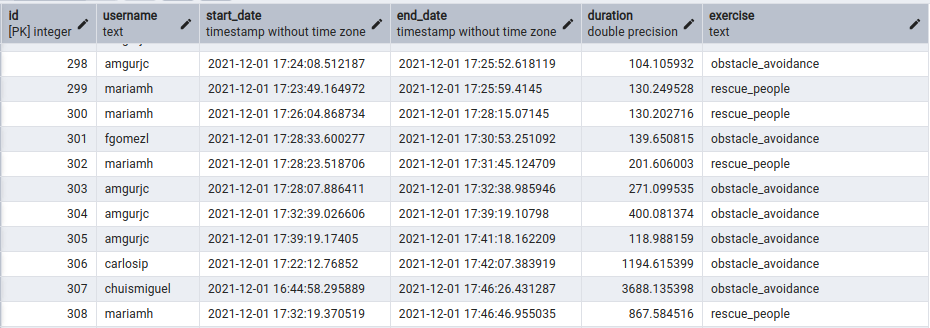
\includegraphics[width=9cm, keepaspectratio]{TFG/2024-tfg-alejandro-aguilera/memoria/img/tablalogejercicios.png}
  \caption{Tabla log\_exercises.}\label{fig:tablalogejercicios}
\end{figure}

La tabla \ref{fig:tablalogejercicios} muestra los registros de las sesiones de ejercicios realizadas por los usuarios. Cada fila representa una sesión, y los campos incluyen información sobre el usuario, el ejercicio realizado, la fecha de inicio y finalización, y la duración de la sesión.

\begin{figure}
  \centering
  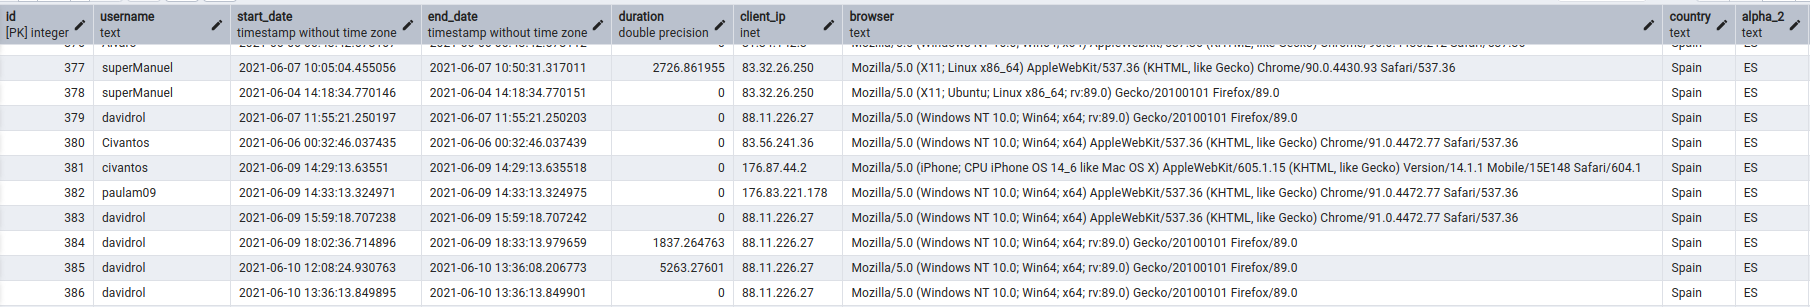
\includegraphics[width=9cm, keepaspectratio]{TFG/2024-tfg-alejandro-aguilera/memoria/img/tablasesiones.png}
  \caption{Tabla log\_session.}\label{fig:tablasesiones}
\end{figure}

La tabla \ref{fig:tablasesiones} contiene información sobre los registros de visitas de los usuarios, incluyendo detalles como el usuario, la fecha de inicio y finalización de la visita, y el navegador y país desde donde se accedió.

\begin{figure}
  \centering
  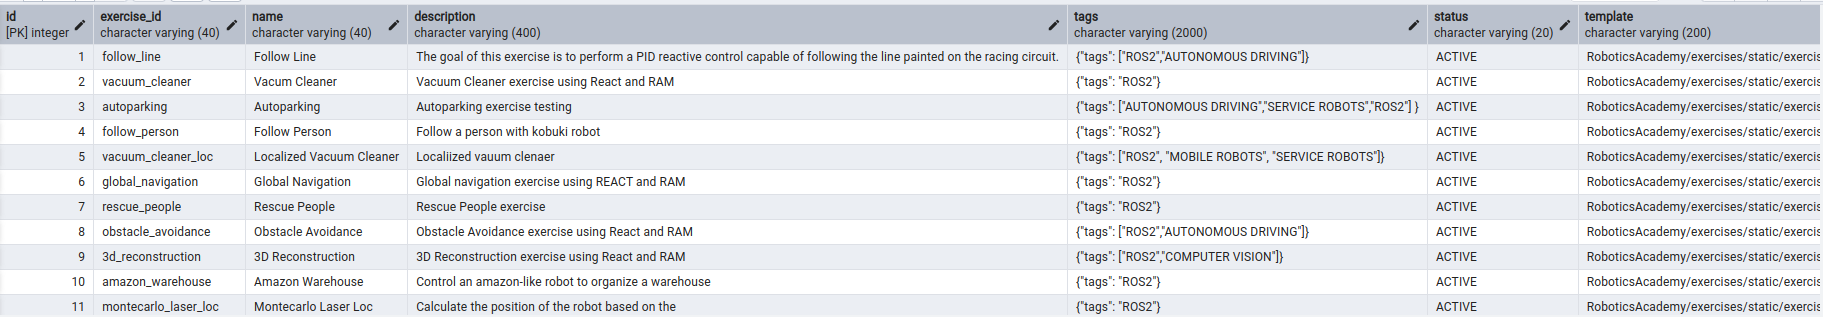
\includegraphics[width=9cm, keepaspectratio]{TFG/2024-tfg-alejandro-aguilera/memoria/img/tablaexercises.png}
  \caption{Tabla exercises.}\label{fig:tablaexercises}
\end{figure}

La tabla \ref{fig:tablaexercises} almacena información sobre los diferentes ejercicios disponibles en la plataforma, como el nombre del ejercicio, su descripción, los tags asociados y su estado. Cada fila de esta tabla corresponde a un ejercicio específico.

\begin{figure}
  \centering
  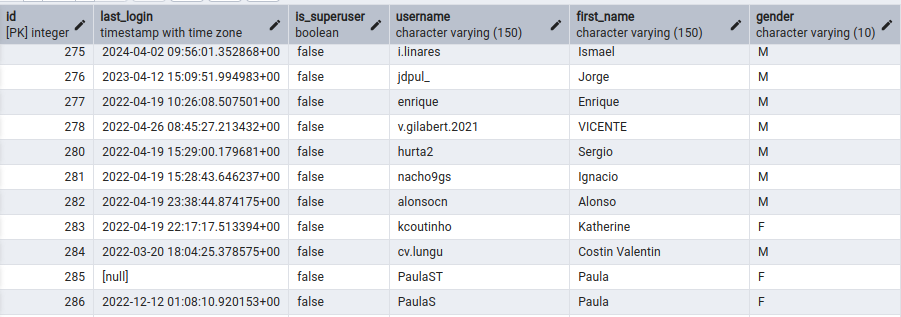
\includegraphics[width=9cm, keepaspectratio]{TFG/2024-tfg-alejandro-aguilera/memoria/img/tablausuarios.png}
  \caption{Tabla common\_user.}\label{fig:tablausuarios}
\end{figure}

La tabla \ref{fig:tablausuarios} contiene información sobre los usuarios registrados en la plataforma, incluyendo su nombre de usuario, nombre real, género, y la última fecha de inicio de sesión. También se almacena si el usuario tiene privilegios de superusuario.

A continuación, ya teniendo en contexto como se almacena la información en las tablas de la base de datos, se presentan ejemplos de consultas SQL que permiten extraer información relevante de las tablas mencionadas anteriormente. Estas consultas pueden ser utilizadas para analizar el comportamiento de los usuarios, las sesiones de ejercicio y el desempeño en los diferentes ejercicios.

y aqui cuando sepa poner codigo pongo querys y explico.
\end{document}

